\documentclass[10pt,fleqn]{article} % Default font size and left-justified equations
\usepackage[%
    pdftitle={Algo : Algorithmes de CPGE},
    pdfauthor={Xavier Pessoles}]{hyperref}

%%%%%%%%%%%%%%%%%%%%%%%%%%%%%%%%%%%%%%%%%
% Original author:
% Mathias Legrand (legrand.mathias@gmail.com) with modifications by:
% Vel (vel@latextemplates.com)
% License:
% CC BY-NC-SA 3.0 (http://creativecommons.org/licenses/by-nc-sa/3.0/)
%%%%%%%%%%%%%%%%%%%%%%%%%%%%%%%%%%%%%%%%%

%----------------------------------------------------------------------------------------
%	VARIOUS REQUIRED PACKAGES AND CONFIGURATIONS
%----------------------------------------------------------------------------------------

% Définition des booleéns
\newif\iffiche
\newif\ifprof
\newif\iftd
\newif\ifcours


\usepackage[top=2.5cm,bottom=2cm,left=2cm,right=2cm,headsep=40pt,a4paper]{geometry} % Page margins

\usepackage{graphicx} % Required for including pictures
\graphicspath{{images/}} % Specifies the directory where pictures are stored

\usepackage{lipsum} % Inserts dummy text

\usepackage{tikz} % Required for drawing custom shapes

\usepackage[french]{babel} % English language/hyphenation
\frenchbsetup{StandardLists=true} % Pour éviter la collision babel enumitem pour les listes

\usepackage{enumitem} % Customize lists
\setlist{nolistsep} % Reduce spacing between bullet points and numbered lists

\usepackage{booktabs} % Required for nicer horizontal rules in tables

\usepackage{colortbl} % Couleur dans les tableaux

\usepackage{xcolor} % Required for specifying colors by name
%\definecolor{ocre}{RGB}{243,102,25} % Define the orange color used for highlighting throughout the book
\definecolor{ocre}{RGB}{49,133,156} % Couleur ''bleue''
\definecolor{violetf}{RGB}{112,48,160} % Couleur ''violet''
\usepackage{enumitem}
\usepackage{pifont} % Pour les dinglist
\usepackage{multicol}
\usepackage{array} % Centrage vertical dans les tableaux

%----------------------------------------------------------------------------------------
%	FONTS
%----------------------------------------------------------------------------------------

\usepackage{avant} % Use the Avantgarde font for headings
%\usepackage{times} % Use the Times font for headings
%\usepackage{mathptmx} % Use the Adobe Times Roman as the default text font together with math symbols from the Sym­bol, Chancery and Com­puter Modern fonts
\usepackage[adobe-utopia]{mathdesign}
\usepackage{microtype} % Slightly tweak font spacing for aesthetics
\usepackage[utf8]{inputenc} % Required for including letters with accents
\usepackage[T1]{fontenc} % Use 8-bit encoding that has 256 glyphs

%----------------------------------------------------------------------------------------
%	BIBLIOGRAPHY AND INDEX
%----------------------------------------------------------------------------------------

\usepackage[style=alphabetic,citestyle=numeric,sorting=nyt,sortcites=true,autopunct=true,babel=hyphen,hyperref=true,abbreviate=false,backref=true,backend=biber]{biblatex}
\addbibresource{bibliography.bib} % BibTeX bibliography file
\defbibheading{bibempty}{}

\usepackage{calc} % For simpler calculation - used for spacing the index letter headings correctly
\usepackage{makeidx} % Required to make an index
\makeindex % Tells LaTeX to create the files required for indexing

%----------------------------------------------------------------------------------------
%	MAIN TABLE OF CONTENTS
%----------------------------------------------------------------------------------------

\usepackage{titletoc} % Required for manipulating the table of contents

\setcounter{tocdepth}{2}     % Dans la table des matieres
\setcounter{secnumdepth}{2}

\contentsmargin{0cm} % Removes the default margin

% Part text styling
\titlecontents{part}[0cm]
{\addvspace{20pt}\centering\large\bfseries}
{}
{}
{}

% Chapter text styling
\titlecontents{chapter}[1.25cm] % Indentation
{\addvspace{12pt}\large\sffamily\bfseries} % Spacing and font options for chapters
{\color{ocre!60}\contentslabel[\Large\thecontentslabel]{1.25cm}\color{ocre}} % Chapter number
{\color{ocre}}  
{\color{ocre!60}\normalsize\;\titlerule*[.5pc]{.}\;\thecontentspage} % Page number

% Section text styling
\titlecontents{section}[1.25cm] % Indentation
{\addvspace{3pt}\sffamily\bfseries} % Spacing and font options for sections
{\color{ocre!60}\contentslabel[\thecontentslabel]{1.25cm} \color{ocre}} % Section number
{\color{ocre}}
{\hfill\color{ocre!60}\thecontentspage} % Page number
[]

% Subsection text styling
\titlecontents{subsection}[1.25cm] % Indentation
{\addvspace{1pt}\sffamily\small} % Spacing and font options for subsections
{\contentslabel[\thecontentslabel]{1.25cm}} % Subsection number
{}
{\ \titlerule*[.5pc]{.}\;\thecontentspage} % Page number
[]


% Subsection text styling
\titlecontents{subsubsection}[1.25cm] % Indentation
{\addvspace{1pt}\sffamily\small} % Spacing and font options for subsections
{\contentslabel[\thecontentslabel]{1.25cm}} % Subsection number
{}
{\ \titlerule*[.5pc]{.}\;\thecontentspage} % Page number
[]

% List of figures
\titlecontents{figure}[0em]
{\addvspace{-5pt}\sffamily}
{\thecontentslabel\hspace*{1em}}
{}
{\ \titlerule*[.5pc]{.}\;\thecontentspage}
[]

% List of tables
\titlecontents{table}[0em]
{\addvspace{-5pt}\sffamily}
{\thecontentslabel\hspace*{1em}}
{}
{\ \titlerule*[.5pc]{.}\;\thecontentspage}
[]

%----------------------------------------------------------------------------------------
%	MINI TABLE OF CONTENTS IN PART HEADS
%----------------------------------------------------------------------------------------

% Chapter text styling
\titlecontents{lchapter}[0em] % Indenting
{\addvspace{15pt}\large\sffamily\bfseries} % Spacing and font options for chapters
{\color{ocre}\contentslabel[\Large\thecontentslabel]{1.25cm}\color{ocre}} % Chapter number
{}  
{\color{ocre}\normalsize\sffamily\bfseries\;\titlerule*[.5pc]{.}\;\thecontentspage} % Page number

% Section text styling
\titlecontents{lsection}[0em] % Indenting
{\sffamily\small} % Spacing and font options for sections
{\contentslabel[\thecontentslabel]{1.25cm}} % Section number
{}
{}

% Subsection text styling
\titlecontents{lsubsection}[.5em] % Indentation
{\normalfont\footnotesize\sffamily} % Font settings
{}
{}
{}

%----------------------------------------------------------------------------------------
%	PAGE HEADERS
%----------------------------------------------------------------------------------------

\usepackage{fancyhdr} % Required for header and footer configuration



\pagestyle{fancy}
 \renewcommand{\headrulewidth}{0pt}
 \fancyhead{}
 \fancyhead[L]{%
 \noindent\begin{minipage}[c]{2.6cm}%
 
\includegraphics[width=2cm]{png/logo_lycee.png}%
 \end{minipage}}

\fancyhead[C]{\rule{8cm}{.5pt}}

 \fancyhead[R]{%
 \noindent\begin{minipage}[c]{3cm}
 \begin{flushright}
 \footnotesize{\textit{\textsf{\xxtete}}}%
 \end{flushright}
 \end{minipage}
}


\fancyfoot[C]{\rule{12cm}{.5pt}}
\renewcommand{\footrulewidth}{0.2pt}
\fancyfoot[C]{\footnotesize{\bfseries \thepage}}
\fancyfoot[L]{ 
\begin{minipage}[c]{.2\linewidth}
\noindent\footnotesize{{\xxauteur}}
\end{minipage}}


\fancyfoot[R]{\footnotesize{\xxpied}
\ifthenelse{\isodd{\value{page}}}{
\begin{tikzpicture}[overlay]
\node[shape=rectangle, 
      rounded corners = .25 cm,
	  draw= ocre,
	  line width=2pt, 
	  fill = ocre!10,
	  minimum width  = 2.5cm,
	  minimum height = 3cm,] at (\xxposongletx,\xxposonglety) {};
\node at (\xxposonglettext,\xxposonglety) {\rotatebox{90}{\textbf{\large\color{ocre}{\xxonglet}}}};
%{};
\end{tikzpicture}}{}
}
%
%
%
% Removes the header from odd empty pages at the end of chapters
\makeatletter
\renewcommand{\cleardoublepage}{
\clearpage\ifodd\c@page\else
\hbox{}
\vspace*{\fill}
\thispagestyle{empty}
\newpage
\fi}

\fancypagestyle{plain}{%
\fancyhf{} % vide l’en-tête et le pied~de~page.
%\fancyfoot[C]{\bfseries \thepage} % numéro de la page en cours en gras
% et centré en pied~de~page.
\fancyfoot[R]{\footnotesize{\xxpied}}
\fancyfoot[C]{\rule{12cm}{.5pt}}
\renewcommand{\footrulewidth}{0.2pt}
\fancyfoot[C]{\footnotesize{\bfseries \thepage}}
\fancyfoot[L]{ 
\begin{minipage}[c]{.2\linewidth}
\noindent\footnotesize{{\xxauteur}}
\end{minipage}}}



%----------------------------------------------------------------------------------------
%	THEOREM STYLES
%----------------------------------------------------------------------------------------

% Conflit avec la police adobe
%\usepackage{amsmath,amsfonts,amssymb,amsthm} % For math equations, theorems, symbols, etc
\usepackage{amsmath,amsthm}

\newcommand{\intoo}[2]{\mathopen{]}#1\,;#2\mathclose{[}}
\newcommand{\ud}{\mathop{\mathrm{{}d}}\mathopen{}}
\newcommand{\intff}[2]{\mathopen{[}#1\,;#2\mathclose{]}}
%\newtheorem{notation}{Notation}[chapter]
\newtheorem{notation}{Notation}[section]

% Boxed/framed environments
\newtheoremstyle{ocrenumbox}% % Theorem style name
{0pt}% Space above
{0pt}% Space below
{\normalfont}% % Body font
{}% Indent amount
{\small\bf\sffamily\color{ocre}}% % Theorem head font
{\;}% Punctuation after theorem head
{0.25em}% Space after theorem head
{\small\sffamily\color{ocre}\thmname{#1}\nobreakspace\thmnumber%{\@ifnotempty{#1}{}\@upn{#2}}% Theorem text (e.g. Theorem 2.1)
\thmnote{\nobreakspace\the\thm@notefont\sffamily\bfseries\color{black}---\nobreakspace#3.}} % Optional theorem note
\renewcommand{\qedsymbol}{$\blacksquare$}% Optional qed square


% Boite pour les corriges
\newtheoremstyle{correctionbox}% % Theorem style name
{0pt}% Space above
{0pt}% Space below
{\normalfont}% % Body font
{}% Indent amount
{\small\bf\sffamily\color{violet}}% % Theorem head font
{\;}% Punctuation after theorem head
{0.25em}% Space after theorem head
{\small\sffamily\color{ocre}\thmname{#1}\nobreakspace\thmnumber%{\@ifnotempty{#1}{}\@upn{#2}}% Theorem text (e.g. Theorem 2.1)
\thmnote{\nobreakspace\the\thm@notefont\sffamily\bfseries\color{black}---\nobreakspace#3.}} % Optional theorem note
\renewcommand{\qedsymbol}{$\blacksquare$}% Optional qed square



\newtheoremstyle{blacknumex}% Theorem style name
{5pt}% Space above
{5pt}% Space below
{\normalfont}% Body font
{} % Indent amount
{\small\bf\sffamily}% Theorem head font
{\;}% Punctuation after theorem head
{0.25em}% Space after theorem head
{\small\sffamily{\tiny\ensuremath{\blacksquare}}\nobreakspace\thmname{#1}\nobreakspace\thmnumber%{\@ifnotempty{#1}{}\@upn{#2}}% Theorem text (e.g. Theorem 2.1)
\thmnote{\nobreakspace\the\thm@notefont\sffamily\bfseries---\nobreakspace#3.}}% Optional theorem note

\newtheoremstyle{blacknumbox} % Theorem style name
{0pt}% Space above
{0pt}% Space below
{\normalfont}% Body font
{}% Indent amount
{\small\bf\sffamily}% Theorem head font
{\;}% Punctuation after theorem head
{0.25em}% Space after theorem head
{\small\sffamily\thmname{#1}\nobreakspace 
\thmnote{\nobreakspace\the\thm@notefont\sffamily\bfseries---\nobreakspace#3.}}% Optional theorem note

% Non-boxed/non-framed environments
\newtheoremstyle{ocrenum}% % Theorem style name
{5pt}% Space above
{5pt}% Space below
{\normalfont}% % Body font
{}% Indent amount
{\small\bf\sffamily\color{ocre}}% % Theorem head font
{\;}% Punctuation after theorem head
{0.25em}% Space after theorem head
{\small\sffamily\color{ocre}\thmname{#1}\nobreakspace%\thmnumber{\@ifnotempty{#1}{}\@upn{#2}}% Theorem text (e.g. Theorem 2.1)
\thmnote{\nobreakspace\the\thm@notefont\sffamily\bfseries\color{black}---\nobreakspace#3.}} % Optional theorem note
\renewcommand{\qedsymbol}{$\blacksquare$}% Optional qed square
\makeatother

% Environnement pour les titres de parties
\newtheoremstyle{partiebox} 
{0pt}% Space above
{0pt}% Space below
{\normalfont}% Body font
{}% Indent amount
{\small\bf\sffamily}% Theorem head font
{\;}% Punctuation after theorem head
{0.25em}% Space after theorem head




% Defines the theorem text style for each type of theorem to one of the three styles above
\newcounter{dummy} 
\numberwithin{dummy}{section}
\theoremstyle{ocrenumbox}
%\newtheorem{theoremeT}[dummy]{Théorème}
\newtheorem{theoremeT}[dummy]{Théorème}
\newtheorem{resultatT}[dummy]{Résultat}
\newtheorem{savoirT}[dummy]{Savoir}
\newtheorem{methodeT}[dummy]{Méthode}
\newtheorem{objectifT}[dummy]{Objectif}
%\newtheorem{problem}{Problem}[chapter]
\newtheorem{problem}{Problem}[section]
%\newtheorem{exerciseT}{Exercise}[chapter]
\newtheorem{exerciseT}{Exercice}[section]

\theoremstyle{blacknumex}
%\newtheorem{exampleT}{Example}[chapter]
\newtheorem{exempleT}{Exemple}[section]
\newtheorem{termT}{Terminal\\}[section]
\newtheorem{pyT}{Python\\}[section]
\newtheorem{sciT}{Scilab\\}[section]
\newtheorem{pseudoT}{Pseudo Code\\}[section]
\newtheorem{sqlT}{SQL\\}[section]

\theoremstyle{blacknumbox}
%\newtheorem{vocabulary}{Vocabulary}[chapter]
\newtheorem{vocabulary}{Vocabulaire}[section]
%\newtheorem{definitionT}{Definition}[section]
\newtheorem{definitionT}{Définition}[section]
\newtheorem{demoT}{Démonstration}[section]
\newtheorem{corollaryT}[dummy]{Corollaire}
\newtheorem{hypoT}{Hypothèse(s)}

\theoremstyle{ocrenum}
\newtheorem{proposition}[dummy]{Proposition}

\theoremstyle{partiebox}
\newtheorem{titrepartieT}[]{}
\newtheorem{titrechapitreT}[]{}

\theoremstyle{correctionbox}
\newtheorem{correctionT}[dummy]{\color{violet}{Correction}}

%----------------------------------------------------------------------------------------
%	DEFINITION OF COLORED BOXES
%----------------------------------------------------------------------------------------

\RequirePackage[framemethod=tikz]{mdframed} % Required for creating the theorem, definition, exercise and corollary boxes

% Theorem box
\newmdenv[skipabove=7pt,
skipbelow=7pt,
backgroundcolor=ocre!10,
linecolor=ocre,
innerleftmargin=5pt,
innerrightmargin=5pt,
innertopmargin=5pt,
leftmargin=0cm,
rightmargin=0cm,
innerbottommargin=5pt]{tBox}


% Correction
\newmdenv[skipabove=7pt,
skipbelow=7pt,
backgroundcolor=violet!10,
linecolor=violet,
innerleftmargin=5pt,
innerrightmargin=5pt,
innertopmargin=5pt,
leftmargin=0cm,
rightmargin=0cm,
innerbottommargin=5pt]{coBox}


% Exercise box	  
\newmdenv[skipabove=7pt,
skipbelow=7pt,
rightline=false,
leftline=true,
topline=false,
bottomline=false,
backgroundcolor=ocre!10,
linecolor=ocre,
innerleftmargin=5pt,
innerrightmargin=5pt,
innertopmargin=5pt,
innerbottommargin=5pt,
leftmargin=0cm,
rightmargin=0cm,
linewidth=4pt]{eBox}	

% Definition box
\newmdenv[skipabove=7pt,
skipbelow=7pt,
rightline=false,
leftline=true,
topline=false,
bottomline=false,
backgroundcolor=ocre!10,
linecolor=ocre,
innerleftmargin=5pt,
innerrightmargin=5pt,
innertopmargin=0pt,
leftmargin=0cm,
rightmargin=0cm,
linewidth=4pt,
innerbottommargin=0pt]{dBox}	

% Demonstration box
\newmdenv[skipabove=7pt,
skipbelow=7pt,
rightline=false,
leftline=true,
topline=false,
bottomline=false,
%backgroundcolor=ocre!10,
linecolor=ocre,
innerleftmargin=5pt,
innerrightmargin=5pt,
innertopmargin=0pt,
leftmargin=0cm,
rightmargin=0cm,
linewidth=4pt,
innerbottommargin=0pt]{demoBox}	

% Corollary box
\newmdenv[skipabove=7pt,
skipbelow=7pt,
rightline=false,
leftline=true,
topline=false,
bottomline=false,
linecolor=gray,
backgroundcolor=black!5,
innerleftmargin=5pt,
innerrightmargin=5pt,
innertopmargin=5pt,
leftmargin=0cm,
rightmargin=0cm,
linewidth=4pt,
innerbottommargin=5pt]{cBox}


% Hypothèses
\newmdenv[skipabove=7pt,
skipbelow=7pt,
rightline=false,
leftline=true,
topline=false,
bottomline=false,
linecolor=gray,
backgroundcolor=black!5,
innerleftmargin=5pt,
innerrightmargin=5pt,
innertopmargin=5pt,
leftmargin=0cm,
rightmargin=0cm,
linewidth=4pt,
innerbottommargin=5pt]{hyBox}


% Boite pour le titre de la partie (pBox)
\newmdenv[skipabove=7pt,
skipbelow=7pt,
rightline=true,
leftline=false,
topline=false,
bottomline=false,
linecolor=ocre,
backgroundcolor=none,
innerleftmargin=5pt,
innerrightmargin=5pt,
innertopmargin=5pt,
leftmargin=0cm,
rightmargin=0cm,
linewidth=4pt,
innerbottommargin=5pt]{pBox}

% Boite pour le titre du chapitre (chBox)
\newmdenv[skipabove=7pt,
skipbelow=7pt,
rightline=false,
leftline=true,
topline=false,
bottomline=false,
linecolor=ocre,
%backgroundcolor=black!5,
innerleftmargin=5pt,
innerrightmargin=5pt,
innertopmargin=5pt,
leftmargin=0cm,
rightmargin=0cm,
linewidth=4pt,
innerbottommargin=5pt]{chBox}


% Boite pour les exemples
\newmdenv[skipabove=7pt,
skipbelow=7pt,
rightline=false,
leftline=true,
topline=false,
bottomline=false,
linecolor=gray,
backgroundcolor=white,
innerleftmargin=5pt,
innerrightmargin=5pt,
innertopmargin=5pt,
leftmargin=0cm,
rightmargin=0cm,
linewidth=4pt,
innerbottommargin=5pt]{exBox}

% Boite pour le terminal
\newmdenv[skipabove=7pt,
skipbelow=7pt,
rightline=false,
leftline=true,
topline=false,
bottomline=false,
linecolor=gray,
backgroundcolor=white,
innerleftmargin=5pt,
innerrightmargin=5pt,
innertopmargin=5pt,
leftmargin=0cm,
rightmargin=0cm,
linewidth=4pt,
innerbottommargin=5pt]{termBox}


% Boite pour Python
\newmdenv[skipabove=7pt,
skipbelow=7pt,
rightline=false,
leftline=true,
topline=false,
bottomline=false,
linecolor=gray,
backgroundcolor=white,
innerleftmargin=5pt,
innerrightmargin=5pt,
innertopmargin=5pt,
leftmargin=0cm,
rightmargin=0cm,
linewidth=4pt,
innerbottommargin=5pt]{pyBox}

% Boite pour scilab
\newmdenv[skipabove=7pt,
skipbelow=7pt,
rightline=false,
leftline=true,
topline=false,
bottomline=false,
linecolor=gray,
backgroundcolor=white,
innerleftmargin=5pt,
innerrightmargin=5pt,
innertopmargin=5pt,
leftmargin=0cm,
rightmargin=0cm,
linewidth=4pt,
innerbottommargin=5pt]{sciBox}


% Boite pour pseudo
\newmdenv[skipabove=7pt,
skipbelow=7pt,
rightline=false,
leftline=true,
topline=false,
bottomline=false,
linecolor=gray,
backgroundcolor=white,
innerleftmargin=5pt,
innerrightmargin=5pt,
innertopmargin=5pt,
leftmargin=0cm,
rightmargin=0cm,
linewidth=4pt,
innerbottommargin=5pt]{pseudoBox}

% Boite pour pseudo
\newmdenv[skipabove=7pt,
skipbelow=7pt,
rightline=false,
leftline=true,
topline=false,
bottomline=false,
linecolor=gray,
backgroundcolor=white,
innerleftmargin=5pt,
innerrightmargin=5pt,
innertopmargin=5pt,
leftmargin=0cm,
rightmargin=0cm,
linewidth=4pt,
innerbottommargin=5pt]{sqlBox}


% Creates an environment for each type of theorem and assigns it a theorem text style from the "Theorem Styles" section above and a colored box from above
\newenvironment{theorem}{\begin{tBox}\begin{theoremeT}}{\end{theoremeT}\end{tBox}}
\newenvironment{resultat}{\begin{tBox}\begin{resultatT}}{\end{resultatT}\end{tBox}}
\newenvironment{methode}{\begin{tBox}\begin{methodeT}}{\end{methodeT}\end{tBox}}
\newenvironment{savoir}{\begin{tBox}\begin{savoirT}}{\end{savoirT}\end{tBox}}
\newenvironment{obj}{\begin{tBox}\begin{objectifT}}{\end{objectifT}\end{tBox}}
\newenvironment{corrige}{\begin{coBox}\begin{correctionT}}{\end{correctionT}\end{coBox}}
\newenvironment{exercise}{\begin{eBox}\begin{exerciseT}}{\hfill{\color{ocre}\tiny\ensuremath{\blacksquare}}\end{exerciseT}\end{eBox}}				  
\newenvironment{exercice}{\begin{eBox}\begin{exerciseT}}{\hfill{\color{ocre}\tiny\ensuremath{\blacksquare}}\end{exerciseT}\end{eBox}}				  

\newenvironment{definition}{\begin{dBox}\begin{definitionT}}{\end{definitionT}\end{dBox}}	
\newenvironment{defi}{\begin{dBox}\begin{definitionT}}{\end{definitionT}\end{dBox}}	
\newenvironment{demo}{\begin{demoBox}\begin{demoT}}{\end{demoT}\end{demoBox}}	
%\newenvironment{exemple}{\begin{exempleT}}{\hfill{\tiny\ensuremath{\blacksquare}}\end{exempleT}}		
\newenvironment{corollary}{\begin{cBox}\begin{corollaryT}}{\end{corollaryT}\end{cBox}}
\newenvironment{hypo}{\begin{hyBox}\begin{hypoT}}{\end{hypoT}\end{hyBox}}	\newenvironment{exemple}{\begin{exBox}\begin{exempleT}}{\hfill{\tiny\ensuremath{\blacksquare}}\end{exempleT}\end{exBox}}	
\newenvironment{titrepartie}{\begin{pBox}\begin{titrepartieT}}{\end{titrepartieT}\end{pBox}}	
\newenvironment{titrechapitre}{\begin{chBox}\begin{titrechapitreT}}{\end{titrechapitreT}\end{chBox}}	

\newenvironment{term}{ \begin{termBox}\begin{termT}}{\end{termT}\end{termBox}}
\newenvironment{py}{ \begin{pyBox}\begin{pyT}}{\end{pyT}\end{pyBox}}
\newenvironment{sci}{ \begin{sciBox}\begin{sciT}}{\end{sciT}\end{sciBox}}
\newenvironment{pseudo}{ \begin{pseudoBox}\begin{pseudoT}}{\end{pseudoT}\end{pseudoBox}}
\newenvironment{envsql}{ \begin{sqlBox}\begin{sqlT}}{\end{sqlT}\end{sqlBox}}


%----------------------------------------------------------------------------------------
%	REMARK ENVIRONMENT
%----------------------------------------------------------------------------------------

\newenvironment{remark}{\par\vspace{10pt}\small % Vertical white space above the remark and smaller font size
\begin{list}{}{
\leftmargin=35pt % Indentation on the left
\rightmargin=25pt}\item\ignorespaces % Indentation on the right
\makebox[-2.5pt]{\begin{tikzpicture}[overlay]
\node[draw=ocre!60,line width=1pt,circle,fill=ocre!25,font=\sffamily\bfseries,inner sep=2pt,outer sep=0pt] at (-15pt,0pt){\textcolor{ocre}{R}};\end{tikzpicture}} % Orange R in a circle
\advance\baselineskip -1pt}{\end{list}\vskip5pt} % Tighter line spacing and white space after remark

\newenvironment{rem}{\par\vspace{10pt}\small % Vertical white space above the remark and smaller font size
\begin{list}{}{
\leftmargin=35pt % Indentation on the left
\rightmargin=25pt}\item\ignorespaces % Indentation on the right
\makebox[-2.5pt]{\begin{tikzpicture}[overlay]
\node[draw=ocre!60,line width=1pt,circle,fill=ocre!25,font=\sffamily\bfseries,inner sep=2pt,outer sep=0pt] at (-15pt,0pt){\textcolor{ocre}{R}};\end{tikzpicture}} % Orange R in a circle
\advance\baselineskip -1pt}{\end{list}\vskip5pt} % Tighter line spacing and white space after remark


\newenvironment{warn}{\par\vspace{10pt}\small % Vertical white space above the remark and smaller font size
\begin{list}{}{
\leftmargin=35pt % Indentation on the left
\rightmargin=25pt}\item\ignorespaces % Indentation on the right
\makebox[-2.5pt]{\begin{tikzpicture}[overlay]
\node[draw=red!60,line width=1pt,circle,fill=red!25,font=\sffamily\bfseries,inner sep=2pt,outer sep=0pt] at (-15pt,0pt){\textcolor{black}{!}};\end{tikzpicture}} % Point d'exclamation dans un cercle
\advance\baselineskip -1pt}{\end{list}\vskip5pt} % Tighter line spacing and white space after remark


%----------------------------------------------------------------------------------------
%	SECTION NUMBERING IN THE MARGIN
%----------------------------------------------------------------------------------------
\setcounter{secnumdepth}{3}
\setcounter{tocdepth}{2}



\makeatletter
\renewcommand{\@seccntformat}[1]{\llap{\textcolor{ocre}{\csname the#1\endcsname}\hspace{1em}}}                    
\renewcommand{\section}{\@startsection{section}{1}{\z@}
{-4ex \@plus -1ex \@minus -.4ex}
{1ex \@plus.2ex }
{\normalfont\large\sffamily\bfseries}}
\renewcommand{\subsection}{\@startsection {subsection}{2}{\z@}
{-3ex \@plus -0.1ex \@minus -.4ex}
{0.5ex \@plus.2ex }
{\normalfont\sffamily\bfseries}}
\renewcommand{\subsubsection}{\@startsection {subsubsection}{3}{\z@}
{-2ex \@plus -0.1ex \@minus -.2ex}
{.2ex \@plus.2ex }
{\normalfont\small\sffamily\bfseries}}                        
\renewcommand\paragraph{\@startsection{paragraph}{4}{\z@}
{-2ex \@plus-.2ex \@minus .2ex}
{.1ex}
{\normalfont\small\sffamily\bfseries}}

%----------------------------------------------------------------------------------------
%	PART HEADINGS
%----------------------------------------------------------------------------------------


%----------------------------------------------------------------------------------------
%	CHAPTER HEADINGS
%----------------------------------------------------------------------------------------

% \newcommand{\thechapterimage}{}%
% \newcommand{\chapterimage}[1]{\renewcommand{\thechapterimage}{#1}}%
% \def\@makechapterhead#1{%
% {\parindent \z@ \raggedright \normalfont
% \ifnum \c@secnumdepth >\m@ne
% \if@mainmatter
% \begin{tikzpicture}[remember picture,overlay]
% \node at (current page.north west)
% {\begin{tikzpicture}[remember picture,overlay]
% \node[anchor=north west,inner sep=0pt] at (0,0) {\includegraphics[width=\paperwidth]{\thechapterimage}};
% \draw[anchor=west] (\Gm@lmargin,-9cm) node [line width=2pt,rounded corners=15pt,draw=ocre,fill=white,fill opacity=0.5,inner sep=15pt]{\strut\makebox[22cm]{}};
% \draw[anchor=west] (\Gm@lmargin+.3cm,-9cm) node {\huge\sffamily\bfseries\color{black}\thechapter. #1\strut};
% \end{tikzpicture}};
% \end{tikzpicture}
% \else
% \begin{tikzpicture}[remember picture,overlay]
% \node at (current page.north west)
% {\begin{tikzpicture}[remember picture,overlay]
% \node[anchor=north west,inner sep=0pt] at (0,0) {\includegraphics[width=\paperwidth]{\thechapterimage}};
% \draw[anchor=west] (\Gm@lmargin,-9cm) node [line width=2pt,rounded corners=15pt,draw=ocre,fill=white,fill opacity=0.5,inner sep=15pt]{\strut\makebox[22cm]{}};
% \draw[anchor=west] (\Gm@lmargin+.3cm,-9cm) node {\huge\sffamily\bfseries\color{black}#1\strut};
% \end{tikzpicture}};
% \end{tikzpicture}
% \fi\fi\par\vspace*{270\p@}}}

%-------------------------------------------

\def\@makeschapterhead#1{%
\begin{tikzpicture}[remember picture,overlay]
\node at (current page.north west)
{\begin{tikzpicture}[remember picture,overlay]
\node[anchor=north west,inner sep=0pt] at (0,0) {\includegraphics[width=\paperwidth]{\thechapterimage}};
\draw[anchor=west] (\Gm@lmargin,-9cm) node [line width=2pt,rounded corners=15pt,draw=ocre,fill=white,fill opacity=0.5,inner sep=15pt]{\strut\makebox[22cm]{}};
\draw[anchor=west] (\Gm@lmargin+.3cm,-9cm) node {\huge\sffamily\bfseries\color{black}#1\strut};
\end{tikzpicture}};
\end{tikzpicture}
\par\vspace*{270\p@}}
\makeatother

%----------------------------------------------------------------------------------------
%	HYPERLINKS IN THE DOCUMENTS
%----------------------------------------------------------------------------------------


\hypersetup{hidelinks,backref=true,pagebackref=true,hyperindex=true,colorlinks=false,breaklinks=true,urlcolor= ocre,bookmarks=true,bookmarksopen=false,pdftitle={Title},pdfauthor={Author}}
\usepackage{bookmark}
\bookmarksetup{
open,
numbered,
addtohook={%
\ifnum\bookmarkget{level}=0 % chapter
\bookmarksetup{bold}%
\fi
\ifnum\bookmarkget{level}=-1 % part
\bookmarksetup{color=ocre,bold}%
\fi
}
}

%----------------------------------------------------------------------------------------
%	
%----------------------------------------------------------------------------------------

\newcommand{\thechapterimage}{}%
\newcommand{\chapterimage}[1]{\renewcommand{\thechapterimage}{#1}}%
\def\@makechapterhead#1{%
{\parindent \z@ \raggedright \normalfont
\begin{tikzpicture}[remember picture,overlay]
\node at (current page.north west)
{\begin{tikzpicture}[remember picture,overlay]
\node[anchor=north west,inner sep=0pt] at (0,0) {\includegraphics[width=\paperwidth]{\thechapterimage}};
%\draw[anchor=west] (\Gm@lmargin,-9cm) node [line width=2pt,rounded corners=15pt,draw=ocre,fill=white,fill opacity=0.5,inner sep=15pt]{\strut\makebox[22cm]{}};
%\draw[anchor=west] (\Gm@lmargin+.3cm,-9cm) node {\huge\sffamily\bfseries\color{black}\thechapter. #1\strut};
\end{tikzpicture}};
\end{tikzpicture}
\par\vspace*{270\p@}
}}




\makeatletter             
\renewcommand{\subparagraph}{\@startsection{subparagraph}{5}{\z@}%
                                    {-2ex \@plus-.2ex \@minus .2ex}%
                                    {0ex}%               
{\normalfont\bfseries Question \hspace{.7cm} }}
\makeatother
\renewcommand{\thesubparagraph}{\arabic{subparagraph}} 
\makeatletter


%%%% Environnement pour inclure du code
\usepackage{textcomp}
\usepackage[french]{algorithm2e}
\usepackage{listings}
\lstloadlanguages{R}   % pour regler les pb d accent utf8 dans les codes
\lstset{language=R} % pour regler les pb d accent utf8 dans les codes
\renewcommand{\lstlistlistingname}{Listings}
\renewcommand{\lstlistingname}{Listing}

\SetKwBlock{Fonction}{Début Fonction}{Fin Fonction}
\SetKwComment{Comment}{start}{end}

\definecolor{Bleu}{rgb}{0.1,0.1,1.0}
\definecolor{Noir}{rgb}{0,0,0}
\definecolor{Grau}{rgb}{0.5,0.5,0.5}
\definecolor{DunkelGrau}{rgb}{0.15,0.15,0.15}
\definecolor{Hellbraun}{rgb}{0.5,0.25,0.0}
\definecolor{Magenta}{rgb}{1.0,0.0,1.0}
\definecolor{Gris}{gray}{0.5}
\definecolor{Vert}{rgb}{0,0.5,0}
\definecolor{SourceHintergrund}{rgb}{1,1.0,0.95}


\lstnewenvironment{python}[1][]{
\lstset{
%escapeinside={\%*}{*)},
inputencoding=utf8,   % pour regler les pb d accent utf8 dans les codes
extendedchars=true,   % pour regler les pb d accent utf8 dans les codes
language=python,
basicstyle=\sffamily\footnotesize, 	
stringstyle=\color{red}, 
showstringspaces=false, 
alsoletter={1234567890},
otherkeywords={\ , \}, \{},
keywordstyle=\color{blue},
emph={access,and,break,class,continue,def,del,elif ,else,
except,exec,finally,for,from,global,if,import,in,i s,
lambda,not,or,pass,print,raise,return,try,while},
emphstyle=\color{black}\bfseries,
emph={[2]True, False, None, self},
emphstyle=[2]\color{black},
emph={[3]from, import, as},
emphstyle=[3]\color{blue},
upquote=true,
columns=flexible, % pour empecher d'avoir un espacement mono
morecomment=[s]{"""}{"""},
commentstyle=\color{Hellbraun}\slshape, 
%emph={[4]1, 2, 3, 4, 5, 6, 7, 8, 9, 0},
emphstyle=[4]\color{blue},
literate=*{:}{{\textcolor{blue}:}}{1}
{=}{{\textcolor{blue}=}}{1}
{-}{{\textcolor{blue}-}}{1}
{+}{{\textcolor{blue}+}}{1}
{*}{{\textcolor{blue}*}}{1}
{!}{{\textcolor{blue}!}}{1}
{(}{{\textcolor{blue}(}}{1}
{)}{{\textcolor{blue})}}{1}
{[}{{\textcolor{blue}[}}{1}
{]}{{\textcolor{blue}]}}{1}
{<}{{\textcolor{blue}<}}{1}
{>}{{\textcolor{blue}>}}{1}
{COMPLETER}{{\textcolor{red}COMPLETER}}{1},
literate=%
            {é}{{\'{e}}}1
            {è}{{\`{e}}}1
            {ê}{{\^{e}}}1
            {ë}{{\¨{e}}}1
            {û}{{\^{u}}}1
            {ù}{{\`{u}}}1
            {â}{{\^{a}}}1
            {à}{{\`{a}}}1
            {î}{{\^{i}}}1
            {ç}{{\c{c}}}1
            {Ç}{{\c{C}}}1
            {É}{{\'{E}}}1
            {Ê}{{\^{E}}}1
            {À}{{\`{A}}}1
            {Â}{{\^{A}}}1
            {Î}{{\^{I}}}1, % pour regler les pb d accent utf8 dans les codes
%framexleftmargin=1mm, framextopmargin=1mm, frame=shadowbox, rulesepcolor=\color{blue},#1
%backgroundcolor=\color{SourceHintergrund}, 
%framexleftmargin=1mm, framexrightmargin=1mm, framextopmargin=1mm, frame=single, framerule=1pt, rulecolor=\color{black},#1
}}{}



\lstnewenvironment{scilab}[1][]{
\lstset{
language=scilab,
basicstyle=\sffamily\footnotesize, 	
stringstyle=\color{red}, 
showstringspaces=false, 
alsoletter={1234567890},
otherkeywords={\ , \}, \{},
keywordstyle=\color{blue},
emph={access,and,break,class,continue,def,del,elif ,else,
except,exec,finally,for,from,global,if,import,in,i s,
lambda,not,or,pass,print,raise,return,try,while,Debut},
emphstyle=\color{black}\bfseries,
emph={[2]True, False, None, self},
emphstyle=[2]\color{black},
emph={[3]from, import, as},
emphstyle=[3]\color{blue},
upquote=true,
columns=flexible, % pour empecher d'avoir un espacement mono
morecomment=[s]{"""}{"""},
commentstyle=\color{Hellbraun}\slshape, 
%emph={[4]1, 2, 3, 4, 5, 6, 7, 8, 9, 0},
emphstyle=[4]\color{blue},
literate=*{:}{{\textcolor{blue}:}}{1}
{=}{{\textcolor{blue}=}}{1}
{-}{{\textcolor{blue}-}}{1}
{+}{{\textcolor{blue}+}}{1}
{*}{{\textcolor{blue}*}}{1}
{!}{{\textcolor{blue}!}}{1}
{(}{{\textcolor{blue}(}}{1}
{)}{{\textcolor{blue})}}{1}
{[}{{\textcolor{blue}[}}{1}
{]}{{\textcolor{blue}]}}{1}
{<}{{\textcolor{blue}<}}{1}
{>}{{\textcolor{blue}>}}{1},
%framexleftmargin=1mm, framextopmargin=1mm, frame=shadowbox, rulesepcolor=\color{blue},#1
%backgroundcolor=\color{SourceHintergrund}, 
%framexleftmargin=1mm, framexrightmargin=1mm, framextopmargin=1mm, frame=single, framerule=1pt, rulecolor=\color{black},#1
}}{}


\lstdefinestyle{stylepython}{%
escapeinside={\%*}{*)},
inputencoding=utf8,   % pour regler les pb d accent utf8 dans les codes
extendedchars=true,   % pour regler les pb d accent utf8 dans les codes
language=python,
basicstyle=\sffamily\footnotesize, 	
stringstyle=\color{red}, 
showstringspaces=false, 
alsoletter={1234567890},
otherkeywords={\ , \}, \{},
keywordstyle=\color{blue},
emph={access,and,break,class,continue,def,del,elif ,else,
except,exec,finally,for,from,global,if,import,in,i s,
lambda,not,or,pass,print,raise,return,try,while},
emphstyle=\color{black}\bfseries,
emph={[2]True, False, None, self},
emphstyle=[2]\color{green},
emph={[3]from, import, as},
emphstyle=[3]\color{blue},
upquote=true,
columns=flexible, % pour empecher d'avoir un espacement mono
morecomment=[s]{"""}{"""},
commentstyle=\color{Hellbraun}\slshape, 
%emph={[4]1, 2, 3, 4, 5, 6, 7, 8, 9, 0},
emphstyle=[4]\color{blue},
literate=*{:}{{\textcolor{blue}:}}{1}
{=}{{\textcolor{blue}=}}{1}
{-}{{\textcolor{blue}-}}{1}
{+}{{\textcolor{blue}+}}{1}
{*}{{\textcolor{blue}*}}{1}
{!}{{\textcolor{blue}!}}{1}
{(}{{\textcolor{blue}(}}{1}
{)}{{\textcolor{blue})}}{1}
{[}{{\textcolor{blue}[}}{1}
{]}{{\textcolor{blue}]}}{1}
{<}{{\textcolor{blue}<}}{1}
{>}{{\textcolor{blue}>}}{1}
{COMPLETER}{{\textcolor{red}COMPLETER}}{1},
literate=%
            {é}{{\'{e}}}1
            {è}{{\`{e}}}1
            {ê}{{\^{e}}}1
            {ë}{{\¨{e}}}1
            {û}{{\^{u}}}1
            {ù}{{\`{u}}}1
            {â}{{\^{a}}}1
            {à}{{\`{a}}}1
            {î}{{\^{i}}}1
            {ç}{{\c{c}}}1
            {Ç}{{\c{C}}}1
            {É}{{\'{E}}}1
            {Ê}{{\^{E}}}1
            {À}{{\`{A}}}1
            {Â}{{\^{A}}}1
            {Î}{{\^{I}}}1,
%numbers=left,                    % where to put the line-numbers; possible values are (none, left, right)
%numbersep=5pt,                   % how far the line-numbers are from the code
%numberstyle=\tiny\color{mygray}, % the style that is used for the line-numbers
}



\lstnewenvironment{termi}[1][]{
\lstset{
language=scilab,
basicstyle=\sffamily\footnotesize, 	
stringstyle=\color{red}, 
showstringspaces=false, 
alsoletter={1234567890},
otherkeywords={\ , \}, \{},
keywordstyle=\color{blue},
emph={access,and,break,class,continue,def,del,elif ,else,
except,exec,finally,for,from,global,if,import,in,i s,
lambda,not,or,pass,print,raise,return,try,while,Debut},
emphstyle=\color{black}\bfseries,
emph={[2]True, False, None, self},
emphstyle=[2]\color{green},
emph={[3]from, import, as},
emphstyle=[3]\color{blue},
upquote=true,
columns=flexible, % pour empecher d'avoir un espacement mono
morecomment=[s]{"""}{"""},
commentstyle=\color{Hellbraun}\slshape, 
%emph={[4]1, 2, 3, 4, 5, 6, 7, 8, 9, 0},
emphstyle=[4]\color{blue},
literate=*{:}{{\textcolor{blue}:}}{1}
{=}{{\textcolor{blue}=}}{1}
{-}{{\textcolor{blue}-}}{1}
{+}{{\textcolor{blue}+}}{1}
{*}{{\textcolor{blue}*}}{1}
{!}{{\textcolor{blue}!}}{1}
{(}{{\textcolor{blue}(}}{1}
{)}{{\textcolor{blue})}}{1}
{[}{{\textcolor{blue}[}}{1}
{]}{{\textcolor{blue}]}}{1}
{<}{{\textcolor{blue}<}}{1}
{>}{{\textcolor{blue}>}}{1},
%framexleftmargin=1mm, framextopmargin=1mm, frame=shadowbox, rulesepcolor=\color{blue},#1
%backgroundcolor=\color{SourceHintergrund}, 
%framexleftmargin=1mm, framexrightmargin=1mm, framextopmargin=1mm, frame=single, framerule=1pt, rulecolor=\color{black},#1
}}{}


\lstnewenvironment{sql}[1][]{
\lstset{
%escapeinside={\%*}{*)},
%inputencoding=utf8,   % pour regler les pb d accent utf8 dans les codes
%extendedchars=true,   % pour regler les pb d accent utf8 dans les codes
language=sql,
basicstyle=\sffamily\footnotesize, 	
stringstyle=\color{red}, 
showstringspaces=false, 
alsoletter={1234567890},
otherkeywords={\ , \}, \{},
keywordstyle=\color{blue},
emph={access,and,break,class,continue,def,del,elif ,else,
except,exec,finally,for,from,global,if,import,in,i s,
lambda,not,or,pass,print,raise,return,try,while},
emphstyle=\color{black}\bfseries,
emph={[2]True, False, None, self},
emphstyle=[2]\color{black},
emph={[3]from, import, as},
emphstyle=[3]\color{blue},
upquote=true,
columns=flexible, % pour empecher d'avoir un espacement mono
morecomment=[s]{"""}{"""},
commentstyle=\color{Hellbraun}\slshape, 
%emph={[4]1, 2, 3, 4, 5, 6, 7, 8, 9, 0},
emphstyle=[4]\color{blue},
literate=*{:}{{\textcolor{blue}:}}{1}
{=}{{\textcolor{blue}=}}{1}
{-}{{\textcolor{blue}-}}{1}
{+}{{\textcolor{blue}+}}{1}
{*}{{\textcolor{blue}*}}{1}
{!}{{\textcolor{blue}!}}{1}
{(}{{\textcolor{blue}(}}{1}
{)}{{\textcolor{blue})}}{1}
{[}{{\textcolor{blue}[}}{1}
{]}{{\textcolor{blue}]}}{1}
{<}{{\textcolor{blue}<}}{1}
{>}{{\textcolor{blue}>}}{1}
{COMPLETER}{{\textcolor{red}COMPLETER}}{1},
literate=%
            {é}{{\'{e}}}1
            {è}{{\`{e}}}1
            {ê}{{\^{e}}}1
            {ë}{{\¨{e}}}1
            {û}{{\^{u}}}1
            {ù}{{\`{u}}}1
            {â}{{\^{a}}}1
            {à}{{\`{a}}}1
            {î}{{\^{i}}}1
            {ç}{{\c{c}}}1
            {Ç}{{\c{C}}}1
            {É}{{\'{E}}}1
            {Ê}{{\^{E}}}1
            {À}{{\`{A}}}1
            {Â}{{\^{A}}}1
            {Î}{{\^{I}}}1, % pour regler les pb d accent utf8 dans les codes
%framexleftmargin=1mm, framextopmargin=1mm, frame=shadowbox, rulesepcolor=\color{blue},#1
%backgroundcolor=\color{SourceHintergrund}, 
%framexleftmargin=1mm, framexrightmargin=1mm, framextopmargin=1mm, frame=single, framerule=1pt, rulecolor=\color{black},#1
}}{}



%%%%%%%%%%%%
% Définition des vecteurs 
%%%%%%%%%%%%
 \newcommand{\vect}[1]{\overrightarrow{#1}}
\newcommand{\axe}[2]{\left(#1,\vect{#2}\right)}

\newcommand{\rep}[1]{\mathcal{R}_{#1}}
\newcommand{\vx}[1]{\vect{x_{#1}}}
\newcommand{\vy}[1]{\vect{y_{#1}}}
\newcommand{\vz}[1]{\vect{z_{#1}}}

%%%%%%%%%%%%
% Définition des torseurs 
%%%%%%%%%%%%

 \newcommand{\torseur}[1]{%
\left\{{#1}\right\}
}

\newcommand{\torseurcin}[3]{%
\left\{\mathcal{#1} \left(#2/#3 \right) \right\}
}

\newcommand{\torseurstat}[3]{%
\left\{\mathcal{#1} \left(#2\rightarrow #3 \right) \right\}
}

 \newcommand{\torseurc}[8]{%
%\left\{#1 \right\}=
\left\{
{#1}
\right\}
 = 
\left\{%
\begin{array}{cc}%
{#2} & {#5}\\%
{#3} & {#6}\\%
{#4} & {#7}\\%
\end{array}%
\right\}_{#8}%
}

 \newcommand{\torseurcol}[7]{
\left\{%
\begin{array}{cc}%
{#1} & {#4}\\%
{#2} & {#5}\\%
{#3} & {#6}\\%
\end{array}%
\right\}_{#7}%
}

 \newcommand{\torseurl}[3]{%
%\left\{\mathcal{#1}\right\}_{#2}=%
\left\{%
\begin{array}{l}%
{#1} \\%
{#2} %
\end{array}%
\right\}_{#3}%
}

 \newcommand{\vectv}[3]{%
\vect{V\left( {#1} \in {#2}/{#3}\right)}
}


\newcommand{\vectf}[2]{%
\vect{R\left( {#1} \rightarrow {#2}\right)}
}

\newcommand{\vectm}[3]{%
\vect{\mathcal{M}\left( {#1}, {#2} \rightarrow {#3}\right)}
}


 \newcommand{\vectg}[3]{%
\vect{\Gamma \left( {#1} \in {#2}/{#3}\right)}
}

 \newcommand{\vecto}[2]{%
\vect{\Omega\left( {#1}/{#2}\right)}
}
% }$$\left\{\mathcal{#1} \right\}_{#2} =%
% \left\{%
% \begin{array}{c}%
%  #3 \\%
%  #4 %
% \end{array}%
% \right\}_{#5}}

%\fichetrue
%\fichefalse

%\proftrue
\proffalse

%\tdtrue
\tdfalse

\courstrue
%\coursfalse

% -------------------------------------
% Déclaration des titres
% -------------------------------------

\def\discipline{Informatique}
\def\xxtete{Informatique}

\def\classe{PTSI}
\def\xxnumpartie{Partie 2}
\def\xxpartie{Algorithmique et Programmation}

\def\xxnumchapitre{Bilan}
\def\xxchapitre{\hspace{.12cm} Algorithmes au programme}

\def\xxposongletx{2}
\def\xxposonglettext{1.45}
\def\xxposonglety{20}
\def\xxonglet{Part. 2 -- Bilan}

\def\xxactivite{Bilan}
\def\xxauteur{\textsl{Xavier Pessoles}}

\def\xxcompetences{%
\textsl{%
\textbf{Savoirs et compétences :}
\begin{itemize}[label=\ding{112},font=\color{ocre}] 
\item Algorithmes
\end{itemize}
%
}}

\def\xxfigures{
%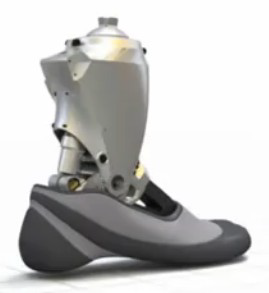
\includegraphics[width=\textwidth]{images/prot_01}

%\textit{Modélisation cinématique} 

}%figues de la page de garde
\def\xxpied{%
Partie 2 -- Algorithmique et Programmation \\
Algorithmes au programme -- \xxactivite%
}

%---------------------------------------------------------------------------


\begin{document}
\chapterimage{png/Fond_ALG}
\pagestyle{empty}


%%%%%%%% PAGE DE GARDE COURS
\ifcours
\begin{tikzpicture}[remember picture,overlay]
\node at (current page.north west)
{\begin{tikzpicture}[remember picture,overlay]
\node[anchor=north west,inner sep=0pt] at (0,0) {\includegraphics[width=\paperwidth]{\thechapterimage}};
\draw[anchor=west] (-2cm,-8cm) node [line width=2pt,rounded corners=15pt,draw=ocre,fill=white,fill opacity=0.6,inner sep=40pt]{\strut\makebox[22cm]{}};
\draw[anchor=west] (1cm,-8cm) node {\huge\sffamily\bfseries\color{black} %
\begin{minipage}{1cm}
\rotatebox{90}{\LARGE\sffamily\textsc{\color{ocre}\textbf{\xxnumpartie}}}
\end{minipage} \hfill
\begin{minipage}[c]{14cm}
\begin{titrepartie}
\begin{flushright}
\renewcommand{\baselinestretch}{1.1} 
\Large\sffamily\textsc{\textbf{\xxpartie}}
\renewcommand{\baselinestretch}{1} 
\end{flushright}
\end{titrepartie}
\end{minipage} \hfill
\begin{minipage}[c]{3.5cm}
{\large\sffamily\textsc{\textbf{\color{ocre} \discipline}}}
\end{minipage} 
 };
\end{tikzpicture}};
\end{tikzpicture}


\begin{tikzpicture}[overlay]
\node[shape=rectangle, 
      rounded corners = .25 cm,
	  draw= ocre,
	  line width=2pt, 
	  fill = ocre!10,
	  minimum width  = 2.5cm,
	  minimum height = 3cm,] at (18cm,0) {};
\node at (17.7cm,0) {\rotatebox{90}{\textbf{\Large\color{ocre}{\classe}}}};
%{};
\end{tikzpicture}

\vspace{3.5cm}

\begin{tikzpicture}[remember picture,overlay]
\draw[anchor=west] (-2cm,-6cm) node {\huge\sffamily\bfseries\color{black} %
\begin{minipage}{2cm}
\begin{center}
\LARGE\sffamily\textsc{\color{ocre}\textbf{\xxactivite}}
\end{center}
\end{minipage} \hfill
\begin{minipage}[c]{15cm}
\begin{titrechapitre}
\renewcommand{\baselinestretch}{1.1} 
\Large\sffamily\textsc{\textbf{\xxnumchapitre}}

\Large\sffamily\textsc{\textbf{\xxchapitre}}
\vspace{.5cm}

\renewcommand{\baselinestretch}{1} 
\normalsize\normalfont
\xxcompetences
\end{titrechapitre}
\end{minipage}  };
\end{tikzpicture}
\vfill

\begin{flushright}
\begin{minipage}[c]{.3\linewidth}
\begin{center}
\xxfigures
\end{center}
\end{minipage}\hfill
\begin{minipage}[c]{.6\linewidth}
\startcontents
\printcontents{}{1}{}
\end{minipage}
\end{flushright}

\begin{tikzpicture}[remember picture,overlay]
\draw[anchor=west] (4.5cm,-.7cm) node {
\begin{minipage}[c]{.2\linewidth}
\begin{flushright}

\includegraphics[width=2cm]{png/logoCC}
\end{flushright}
\end{minipage}
\begin{minipage}[c]{.2\linewidth}
\textsl{\xxauteur} \\
\textsl{\classe}
\end{minipage}
 };
\end{tikzpicture}
\newpage
\pagestyle{fancy}

\newpage
\pagestyle{fancy}

\else
\fi


%%%%%%%% PAGE DE GARDE TD
\iftd
%\begin{tikzpicture}[remember picture,overlay]
%\node at (current page.north west)
%{\begin{tikzpicture}[remember picture,overlay]
%\draw[anchor=west] (-2cm,-3.25cm) node [line width=2pt,rounded corners=15pt,draw=ocre,fill=white,fill opacity=0.6,inner sep=40pt]{\strut\makebox[22cm]{}};
%\draw[anchor=west] (1cm,-3.25cm) node {\huge\sffamily\bfseries\color{black} %
%\begin{minipage}{1cm}
%\rotatebox{90}{\LARGE\sffamily\textsc{\color{ocre}\textbf{\xxnumpartie}}}
%\end{minipage} \hfill
%\begin{minipage}[c]{13.5cm}
%\begin{titrepartie}
%\begin{flushright}
%\renewcommand{\baselinestretch}{1.1} 
%\Large\sffamily\textsc{\textbf{\xxpartie}}
%\renewcommand{\baselinestretch}{1} 
%\end{flushright}
%\end{titrepartie}
%\end{minipage} \hfill
%\begin{minipage}[c]{3.5cm}
%{\large\sffamily\textsc{\textbf{\color{ocre} \discipline}}}
%\end{minipage} 
% };
%\end{tikzpicture}};
%\end{tikzpicture}

%%%%%%%%%% PAGE DE GARDE TD %%%%%%%%%%%%%%%
%\begin{tikzpicture}[overlay]
%\node[shape=rectangle, 
%      rounded corners = .25 cm,
%	  draw= ocre,
%	  line width=2pt, 
%	  fill = ocre!10,
%	  minimum width  = 2.5cm,
%	  minimum height = 2.5cm,] at (18.5cm,0) {};
%\node at (17.7cm,0) {\rotatebox{90}{\textbf{\Large\color{ocre}{\classe}}}};
%%{};
%\end{tikzpicture}

% PARTIE ET CHAPITRE
%\begin{tikzpicture}[remember picture,overlay]
%\draw[anchor=west] (-1cm,-2.1cm) node {\large\sffamily\bfseries\color{black} %
%\begin{minipage}[c]{15cm}
%\begin{flushleft}
%\xxnumchapitre \\
%\xxchapitre
%\end{flushleft}
%\end{minipage}  };
%\end{tikzpicture}

% Bandeau titre exo
\begin{tikzpicture}[remember picture,overlay]
\draw[anchor=west] (-2cm,-6cm) node {\huge\sffamily\bfseries\color{black} %
\begin{minipage}{5cm}
\begin{center}
\LARGE\sffamily\color{ocre}\textbf{\textsc{\xxactivite}}

\begin{center}
\xxfigures
\end{center}

\end{center}
\end{minipage} \hfill
\begin{minipage}[c]{12cm}
\begin{titrechapitre}
\renewcommand{\baselinestretch}{1.1} 
\large\sffamily\textbf{\textsc{\xxtitreexo}}

\small\sffamily{\textbf{\textit{\color{black!70}\xxsourceexo}}}
\vspace{.5cm}

\renewcommand{\baselinestretch}{1} 
\normalsize\normalfont
\xxcompetences
\end{titrechapitre}
\end{minipage}  };
\end{tikzpicture}

\else
\fi


%%%%%%%% PAGE DE GARDE FICHE
\iffiche
\begin{tikzpicture}[remember picture,overlay]
\node at (current page.north west)
{\begin{tikzpicture}[remember picture,overlay]
\draw[anchor=west] (-2cm,-3.25cm) node [line width=2pt,rounded corners=15pt,draw=ocre,fill=white,fill opacity=0.6,inner sep=40pt]{\strut\makebox[22cm]{}};
\draw[anchor=west] (1cm,-3.25cm) node {\huge\sffamily\bfseries\color{black} %
\begin{minipage}{1cm}
\rotatebox{90}{\LARGE\sffamily\textsc{\color{ocre}\textbf{\xxnumpartie}}}
\end{minipage} \hfill
\begin{minipage}[c]{14cm}
\begin{titrepartie}
\begin{flushright}
\renewcommand{\baselinestretch}{1.1} 
\large\sffamily\textsc{\textbf{\xxpartie} \\} 

\vspace{.2cm}

\normalsize\sffamily\textsc{\textbf{\xxnumchapitre -- \xxchapitre}}
\renewcommand{\baselinestretch}{1} 
\end{flushright}
\end{titrepartie}
\end{minipage} \hfill
\begin{minipage}[c]{3.5cm}
{\large\sffamily\textsc{\textbf{\color{ocre} \discipline}}}
\end{minipage} 
 };
\end{tikzpicture}};
\end{tikzpicture}


\begin{tikzpicture}[overlay]
\node[shape=rectangle, 
      rounded corners = .25 cm,
	  draw= ocre,
	  line width=2pt, 
	  fill = ocre!10,
	  minimum width  = 2.5cm,
%	  minimum height = 2.5cm,] at (18.5cm,0.5cm) {};
	  minimum height = 2.5cm,] at (18.5cm,0cm) {};
\node at (17.7cm,0) {\rotatebox{90}{\textsf{\textbf{\large\color{ocre}{\classe}}}}};
%{};
\end{tikzpicture}



\else
\fi




%\newpage

%%%%%%%%%%%%%%%%%  FIN DE LA COPIE *****************



\section{Recherches dans une liste}
\subsection{Recherche d'un nombre dans une liste}

%\subsubsection{Algorithme naïf}

\begin{pseudo}
\begin{center}
\begin{tabular}{p{.9\textwidth}}
\hline
\textbf{Algorithme :} Recherche naïve d'un nombre dans une liste triée ou non \\
\hline
\textbf{Données :}
\begin{itemize}
\item \textsf{n}, int : un entier 
\item \textsf{tab}, liste : une liste d'entiers triés ou non triés
\end{itemize}
\textbf{Résultat :} 
\begin{itemize}
\item un booléen : \textsf{Vrai} si le nombre est dans la liste, \textsf{Faux} sinon.
\end{itemize} \\
\\
\textbf{is\_number\_in\_list}(\textsf{n},\textsf{tab}) :\\
\hspace{.4cm}\textsf{l} $\leftarrow$ \textbf{longueur}(\textsf{tab}) \\
\hspace{.4cm}\textbf{Pour} \textsf{i} \textbf{allant de} 1 \textbf{à} \textsf{l} \textbf{faire} : \\
\hspace{.8cm} \textbf{Si}  \textsf{tab[i] = n} \textbf{alors} :\\
\hspace{1.2cm}\textbf{Retourne} \textsf{Vrai} \\
\hspace{.8cm} \textbf{Fin Si} \\
\hspace{.4cm}\textbf{Fin Faire} \\
\hspace{.4cm}\textbf{Retourne} \textsf{Faux} \\
\textbf{Fin fonction} \\
\hline
\end{tabular}
\end{center}
\end{pseudo}


\begin{minipage}[c]{.49\linewidth}
\begin{py}
\begin{python}
def is_number_in_list(nb,tab):
    """Renvoie True si le nombre nb est dans la liste 
    de nombres tab
    Keyword arguments:
      * nb, int -- nombre entier
      * tab, list -- liste de nombres entiers    
    """
    for i in range(len(tab)):
        if tab[i]==nb:
            return True
    return False
\end{python}
\end{py}
\end{minipage}\hfill
\begin{minipage}[c]{.49\linewidth}
\begin{py}
\begin{python}
def is_number_in_list(nb,tab):
    """Renvoie True si le nombre nb est dans la liste 
    de nombres tab
    Keyword arguments:
      * nb, int -- nombre entier
      * tab, list -- liste de nombres entiers    
    """
    i=0
    while i<len(tab) and tab[i]!=nb:
        i+=1
    return i<len(tab)
\end{python}
\end{py}
\end{minipage}

\begin{rem}
Ces algorithmes sont modifiables aisément dans le cas où on souhaiterait connaître l'index du nombre recherché.
\end{rem}

%\subsubsection{Algorithme raccourci}



\subsection{Recherche du maximum dans une liste de nombre}

\begin{minipage}[c]{.48\linewidth}
\begin{pseudo}
\begin{center}
\begin{tabular}{p{.9\textwidth}}
\hline
\textbf{Algorithme :} Recherche du maximum dans une liste de nombres\\
\hline
\textbf{Données :}
\begin{itemize}
\item \textsf{tab}, liste : une liste de nombres
\end{itemize}
\textbf{Résultat :} 
\begin{itemize}
\item \textsf{maxi}, réel : maximum de la liste
\end{itemize} \\
\\
\textbf{what\_is\_max}(\textsf{tab}) :\\
\hspace{.4cm}\textsf{n} $\leftarrow$ \textbf{longueur}(\textsf{tab}) \\
\hspace{.4cm}\textsf{i  $\leftarrow$ 2} \\
\hspace{.4cm}\textsf{maxi  $\leftarrow$ tab[1]} \\
\hspace{.4cm}\textbf{Tant que} \textsf{i < n} \textbf{faire} : \\
\hspace{.8cm}\textbf{Si} \textsf{tab[i]>maxi} \textbf{alors} : \\
\hspace{1.2cm} \textsf{maxi  $\leftarrow$ tab[i]} \\
\hspace{.8cm}\textbf{Fin si} \\
\hspace{.8cm}\textsf{i  $\leftarrow$ i+1} \\
\hspace{.4cm}\textbf{Fin tant que} \\
\hspace{.4cm}\textbf{Retourner} \textsf{maxi}\\
\textbf{Fin fonction} \\
\hline
\end{tabular}
\end{center}
\end{pseudo}
\end{minipage} \hfill
\begin{minipage}[c]{.48\linewidth}
\begin{py}
\begin{python}
def what_is_max(tab):
    """ 
    Renvoie le plus grand nombre d'une liste
    Keyword arguments:
    tab -- liste de nombres 
    """
    i=1
    maxi=tab[0]
    while i<len(tab):
        if tab[i]>maxi:
            maxi=tab[i]
        i+=1
    return maxi
\end{python}
\end{py}
\end{minipage}

\subsection{Recherche par dichotomie dans un tableau trié}


\begin{minipage}[c]{.48\linewidth}
\begin{pseudo}
\begin{center}
\begin{tabular}{p{.9\textwidth}}
\hline
\textbf{Algorithme :} Recherche par dichotomie d'un nombre dans une liste triée\\
\hline
\textbf{Données :}
\begin{itemize}
\item \textsf{nb}, int : un entier 
\item \textsf{tab}, liste : une liste d'entiers triés
\end{itemize}
\textbf{Résultat :} 
\begin{itemize}
\item \textsf{m}, int : l'index du nombre recherché
\item \textsf{None} : cas où \textsf{nb} n'est pas dans \textsf{tab}
\end{itemize}
\\
\textbf{is\_number\_in\_list\_dicho}(\textsf{nb},\textsf{tab}) :\\
\hspace{.4cm}\textsf{g} $\leftarrow$ \textsf{0} \\
\hspace{.4cm}\textsf{d} $\leftarrow$ \textbf{longueur}(\textsf{tab}) \\
\hspace{.4cm}\textbf{Tant que} \textsf{g $<$ d} \textbf{alors} : \\
\hspace{.8cm} \textsf{m} $\leftarrow$ \textsf{(g+d)} \textbf{div} \textsf{2}\\
\hspace{1.2cm}\textbf{Si} \textsf{tab[m]=nb} \textbf{alors} :\\
\hspace{1.6cm}\textbf{Retourne} \textsf{m}\\
\hspace{1.2cm}\textbf{Sinon si} \textsf{tab[m]<nb} \textbf{alors} :\\
\hspace{1.6cm}\textsf{g} $\leftarrow$ \textsf{m+1}\\
\hspace{1.2cm}\textbf{Sinon, alors} :\\
\hspace{1.6cm}\textsf{d} $\leftarrow$ \textsf{m-1}\\
\hspace{.8cm} \textbf{Fin Si} \\
\hspace{.4cm}\textbf{Fin Tant que} \\
\hspace{.4cm}\textbf{Retourne} \textsf{None} \\
\textbf{Fin fonction} \\
\hline
\end{tabular}
\end{center}
\end{pseudo}
\end{minipage} \hfill
\begin{minipage}[c]{.48\linewidth}
\begin{py}
\begin{python}
def is_number_in_list_dicho(nb,tab):
    """ 
    Recherche d'un nombre par dichotomie dans un 
    tableau trié. 
    Renvoie l'index si le nombre nb est dans la liste 
    de nombres tab.
    Renvoie None sinon.
    Keyword arguments:
    nb,int -- nombre entier
    tab,list -- liste de nombres entiers triés
    """
    g, d = 0, len(tab)-1
    while g <= d:
        m = (g + d) // 2
        if tab[m] == nb:
            return m
        if tab[m] < nb:
            g = m+1
        else:
            d = m-1
    return None
\end{python}
\end{py}
\end{minipage}

\section{Gestion d'une liste de nombres}
\subsection{Calcul de la moyenne}

\begin{minipage}[c]{.48\linewidth}
\begin{pseudo}
\begin{center}
\begin{tabular}{p{.9\textwidth}}
\hline
\textbf{Algorithme :} Calcul de la moyenne arithmétique des nombres d'une liste\\
\hline
\textbf{Données :}
\begin{itemize}
\item \textsf{tab}, liste : une liste de nombres
\end{itemize}
\textbf{Résultat :} 
\begin{itemize}
\item \textsf{res}, réel : moyenne des nombres
\end{itemize} \\
\\
\textbf{calcul\_moyenne}(\textsf{tab}) :\\
\hspace{.4cm}\textsf{n} $\leftarrow$ \textbf{longueur}(\textsf{tab}) \\
\hspace{.4cm}\textsf{res} $\leftarrow$ \textsf{0} \\
\hspace{.4cm}\textbf{Pour} \textsf{i} \textbf{allant de}\textsf{1} \textbf{à} \textsf{n} \textbf{faire}: \\
\hspace{.8cm} \textsf{res  $\leftarrow$ res+tab[i]} \\
\hspace{.4cm}\textbf{Fin faire} \\
\hspace{.4cm}\textbf{Retourner} \textsf{res/n}\\
\textbf{Fin fonction} \\
\hline
\end{tabular}
\end{center}
\end{pseudo}
\end{minipage} \hfill
\begin{minipage}[c]{.48\linewidth}
\begin{py}
\begin{python}
def calcul_moyenne(tab):
    """ 
    Renvoie la moyenne des valeurs d'une liste de 
    nombres.
    Keyword arguments:
    tab -- liste de nombres
    """
    res = 0
    for i in range(len(tab)):
        res = res+tab[i]
    return res/(len(tab))
\end{python}
\end{py}    
\end{minipage}

\newpage

\subsection{Calcul de la variance}
Soit une série statistique prenant les $n$ valeurs $x_1$, $x_2$, ..., $x_n$. Soit $m$ la moyenne de ces valeurs. La variance est définie par :
$$
v = \dfrac{1}{n} \sum\limits_{i=1}^n\left(x_i - m \right)^2
$$


\begin{minipage}[c]{.48\linewidth}
\begin{pseudo}
\begin{center}
\begin{tabular}{p{.9\textwidth}}
\hline
\textbf{Algorithme :} Calcul de la variance des nombres d'une liste\\
\hline
\textbf{Données :}
\begin{itemize}
\item \textsf{tab}, liste : une liste de nombres
\item \textsf{m}, réel : moyenne de la liste
\end{itemize}
\textbf{Résultat :} 
\begin{itemize}
\item \textsf{res}, réel : variance
\end{itemize} \\
\\
\textbf{calcul\_variance}(\textsf{tab}) :\\
\hspace{.4cm}\textsf{n} $\leftarrow$ \textbf{longueur}(\textsf{tab}) \\
\hspace{.4cm}\textsf{res} $\leftarrow$ \textsf{0} \\
\hspace{.4cm}\textbf{Pour} \textsf{i} \textbf{allant de} \textsf{1} \textbf{à} \textsf{n} \textbf{faire}: \\
\hspace{.8cm} \textsf{res  $\leftarrow$ res+(tab[i]-m)**2} \\
\hspace{.4cm}\textbf{Fin faire} \\
\hspace{.4cm}\textbf{Retourner} \textsf{res/n}\\
\textbf{Fin fonction} \\
\hline
\end{tabular}
\end{center}

\end{pseudo}
\end{minipage} \hfill
\begin{minipage}[c]{.48\linewidth}
\begin{py}
\begin{python}
def calcul_variance(tab,m):
    """ 
    Renvoie la variance des valeurs d'un tableau.
    Keyword arguments:
    tab -- liste de nombres
    m -- moyenne des valeurs
    """
    res = 0
    for i in range(len(tab)):
        res = res+(tab[i]-m)**2
    return res/(len(tab))
\end{python}
\end{py}
\end{minipage} 

\subsection{Calcul de la médiane} %Seconde année


\begin{minipage}[c]{.48\linewidth}
\begin{pseudo}
\begin{center}
\begin{tabular}{p{.9\textwidth}}
\hline
\textbf{Algorithme :} Recherche de la valeur médiane d'une liste de nombres triés \\
\hline
\textbf{Données :}
\begin{itemize}
\item \textsf{tab}, liste : liste de nombres triés
\end{itemize}
\textbf{Résultat :} 
\begin{itemize}
\item flt : valeur de la médiane
\end{itemize}
\\
\textbf{mediane}(\textsf{tab}) :\\
\hspace{.4cm}\textsf{n} $\leftarrow$ \textbf{Longueur}\textsf{(tab)} \\
\hspace{.4cm}\textbf{Si} \textsf{n} \textbf{modulo} \textsf{2 = 0} \textbf{Alors} : \\
\hspace{.8cm} \textsf{i $\leftarrow$ n/2} \\
\hspace{.8cm} \textbf{Retourner} \textsf{(tab[i] +tab[i+1])/2} \\
\hspace{.4cm}\textbf{Sinon} :\\
\hspace{.8cm} \textsf{i $\leftarrow$ n}\textbf{div} \textsf{2+1} \\
\hspace{.8cm} \textbf{Retourner} \textsf{(tab[i])} \\
\textbf{Fin fonction} \\
\hline
\end{tabular}
\end{center}
\end{pseudo}
\end{minipage} \hfill
\begin{minipage}[c]{.48\linewidth}
\begin{py}
\begin{python}
def calcul_mediane(tab):
    """ 
    Calcule la variance des éléments d'un tableau trié.
    Keyword arguments:
    tab -- liste de nombres
    """
    if len(tab)%2 == 0 :
        i=len(tab)//2
        return (tab[i-1]+tab[i])/2
    else :
        i = len(tab)//2
    return tab[i]
\end{python}
\end{py}
\end{minipage}
%\subsubsection*{Estimation de la complexité}

\section{Chaînes de caractères}
\subsection{Recherche d'un mot dans une chaîne de caractères}

%\begin{minipage}[c]{.48\linewidth}
%\begin{pseudo}
%\end{pseudo}
%\end{minipage} \hfill
%\begin{minipage}[c]{.48\linewidth}
\begin{py}
\begin{python}
def index_of_word_in_text(mot, texte):
    """ Recherche si le mot est dans le texte.
    Renvoie l'index si le mot est présent, None sinon.
    Keyword arguments:
    mot -- mot recherché
    texte -- texte
    """
    for i in range(1 + len(texte) - len(mot)):
        j = 0
        while j < len(mot) and mot[j] == texte[i + j]:
            j += 1
        if j == len(mot):
            return i
    return None
\end{python}
\end{py}
%\end{minipage}

%\subsubsection*{Estimation de la complexité}

\section{Calcul numérique}
\subsection{Recherche du zéro d'une fonction continue monotone par la méthode de dichotomie}


\begin{minipage}[c]{.48\linewidth}
\begin{pseudo}
\begin{center}
\begin{tabular}{p{.9\textwidth}}
\hline
\textbf{Algorithme :} Recherche de la solution de $f(x)=0$ par dichotomie \\
\hline
\textbf{Données :}
\begin{itemize}
\item \textsf{f}, fonction : fonction continue et monotone sur $[a,b]$
\item \textsf{a, b}, réels : nombre réels tels que $a<b$
\item \textsf{$\varepsilon$}, réel : tolérance du calcul
\end{itemize}
\textbf{Résultat :} 
\begin{itemize}
\item flt : solution de l'équation
\end{itemize}
\\
\textbf{solveDichotomie}(\textsf{f,a,b,$\varepsilon$}) :\\
\hspace{.4cm}\textsf{g} $\leftarrow$ \textsf{a} \\
\hspace{.4cm}\textsf{d} $\leftarrow$ \textsf{b} \\
\hspace{.4cm}\textbf{Tant que} \textsf{d-g>$\varepsilon$} \textbf{Alors} : \\
\hspace{.8cm}\textsf{m} $\leftarrow$ \textsf{(g+d)/2} \\
\hspace{.8cm}\textbf{Si} \textsf{f(g)*f(m) $\leq$ 0} \textbf{Alors} : \\
\hspace{1.2cm}\textsf{d $\leftarrow$  m} \\
\hspace{.8cm} \textbf{Sinon :} \\
\hspace{1.2cm}\textsf{g $\leftarrow$  m} \\
\hspace{.8cm} \textbf{Fin Si}\\
\hspace{.4cm} \textbf{Fin Tant que}\\
\textbf{Fin fonction} \\
\hline
\end{tabular}
\end{center}
\end{pseudo}
%\begin{pseudo}
%\begin{algorithm}[H]
%\Fonction{
%Données:$f$, $a$,$b$, $\varepsilon$ \\
%$g\gets a$\\
%$d \gets b$\\
%$f_g \gets f(g)$\\
%$f_d \gets f(d)$\\
%\Tq{$ (d-g) > \varepsilon$}{
%$m \gets (g+d)/2$ \\
%$f_m\gets f(m)$
%
%\eSi{$f_g\cdot f_m \leq 0$}{
%$d \gets m$\\
%$f_d \gets f_m$\\
%}{
%$g \gets m$\\
%$f_d \gets f_m$\\
%}
%}
%\Retour{$(g+d)/2$}
%}
%\end{algorithm}
%\end{pseudo}
\end{minipage} \hfill
\begin{minipage}[c]{.48\linewidth}
\begin{py}
\begin{python}
def solveDichotomie(f,a,b,eps):
    """
    Recherche par dichotomie de la solution 
    de l'équation f(x)=0.
    Keywords arguments :
    Entrées : 
        a,b, flt : Nombre réels tels que a<b
        f, function : fonction continue et monotone 
        sur [a,b]
        eps,flt : tolérance de la résolution
    Sortie : 
        flt : solution de la fonction
    """
    g = a
    d = b
    while (d-g) > eps:
        m = (g+d)/2 
        if f(g) * f(m) <= 0 :
            d = m
        else :
            g  = m
    return (g+d)/2
\end{python}
\end{py}
\end{minipage}

%\subsubsection*{Précision du calcul}
%\subsubsection*{Rapidité}
%\subsubsection*{Comparaison à zéro}

\subsection{Recherche du zéro d'une fonction continue monotone par la méthode de Newton}


\begin{minipage}[c]{.48\linewidth}
\begin{pseudo}
\begin{center}
\begin{tabular}{p{.9\textwidth}}
\hline
\textbf{Algorithme :} Recherche de la solution de $f(x)=0$ par la méthode de Newton \\
\hline
\textbf{Données :}
\begin{itemize}
\item \textsf{f}, fonction : fonction continue et monotone sur $[a,b]$
\item \textsf{df}, fonction : fonction dérivée de $f$ sur $[a,b]$
\item \textsf{a}, réel : nombre réel tel que
\item \textsf{$\varepsilon$}, réel : tolérance du calcul
\end{itemize}
\textbf{Résultat :} 
\begin{itemize}
\item c: flt : solution de l'équation
\end{itemize}
\\
\textbf{solveNewton}(\textsf{f,df,a,$\varepsilon$}) :\\
\hspace{.4cm} $c \gets  a-\dfrac{f(a)}{df(a)} $\\ 
\hspace{.4cm} \textbf{Tant que} $ |c-a|> \varepsilon$ \textbf{alors} \\
\hspace{.8cm} $a \gets  c$\\
\hspace{.8cm} $c \gets  c-\dfrac{f(c)}{df(c)} $\\ 
\textbf{Fin fonction} \\
\hline
\end{tabular}
\end{center}
%\begin{algorithm}[H]
%\Fonction{
%Données:$f$, $f'$, $a$, $\varepsilon$ \\
%$g\gets a$\\
%$c \gets  g-\dfrac{f(g)}{f'(g)} $\\
%\Tq{$ |c-g|> \varepsilon$}{
%$g \gets  c$ \\
%$c \gets c-\dfrac{f(c)}{f'(c)}$
%}
%\Retour{$c$}
%}
%\end{algorithm}
\end{pseudo}
\end{minipage} \hfill
\begin{minipage}[c]{.48\linewidth}
\begin{py}
\begin{python}
def solveNewton(f,df,a,eps):
    """
    Recherche par la méthode de Newton de la solution 
    de l'équation f(x)=0.
    Keywords arguments :
    Entrées :
        f, function : fonction à valeur de IR dans IR
        df, function : dérivée de f à valeur de IR dans IR
        a, flt : solution initiale
        eps,flt : tolérance de la résolution
    Sortie : 
        m : flt : solution de la fonction    
    """
    c = a-f(a)/df(a)
    while abs(c-a)>eps:
        a = c
        c = c-f(c)/df(c)
    return c
\end{python}
\end{py}
\end{minipage} 

\begin{rem}
La dérivée de $f$ notée $f'$ pourra être une fonction qui a été définie. On peut aussi calculer la dérivée de façon numérique. Ainsi, en tenant compte des précautions mathématiques d'usage, il est possible de procéder ainsi :

\begin{py}
\begin{python}
def derive_fonctions(f,x,eps):
    return (f(x+eps)-f(x))/(eps)
\end{python}
\end{py}
\end{rem}


%\subsubsection*{Précision du calcul}
%\subsubsection*{Rapidité}

\subsection{Méthode des rectangles pour le calcul approché d'une intégrale sur un segment}
\subsubsection{Méthode des rectangles à gauche}

\begin{pseudo}
\begin{center}
\begin{tabular}{p{.9\textwidth}}
\hline
\textbf{Algorithme :} Calcul d'intégrale par la méthode des rectangles à gauche\\
\hline
\textbf{Données :}
\begin{itemize}
\item \textsf{f}, fonction : fonction définie sur $[a,b]$  
\item \textsf{a}, réel : borne inférieure de l'intervalle de définition
\item \textsf{b}, réel : borne supérieure de l'intervalle de définition, \textsf{b$\geq$a}
\item \textsf{nb}, entiers : nombre d'échantillons pour calculer l'intégrale
\end{itemize}
\textbf{Résultat :} 
\begin{itemize}
\item \textsf{res}, réel : valeur approchée de $\int\limits_a^b f(t)\text{d}t$
\end{itemize}
\\
\textbf{integrale\_rectangles\_gauche}(\textsf{f,a,b,nb}) :\\
\hspace{.4cm}\textsf{res} $\leftarrow$ \textsf{0}\\
\hspace{.4cm}\textsf{pas} $\leftarrow$ \textsf{(b-a)/nb}\\
\hspace{.4cm}\textsf{x} $\leftarrow$ \textsf{a}\\
\hspace{.4cm}\textbf{Tant que} \textsf{x<b},  \textbf{Faire :}\\
\hspace{.8cm}\textsf{res}$\leftarrow$ \textsf{res + } \textbf{f(}\textsf{x}\textbf{)}\\
\hspace{.8cm}\textsf{x} $\leftarrow$ \textsf{x+pas}\\
\hspace{.4cm}\textbf{Fin Tant que} \\
\hspace{.4cm} \textsf{res} $\leftarrow$ \textsf{res*pas}\\
\hspace{.4cm}\textbf{Retourner} \textsf{res}\\
\textbf{Fin Fonction} \\
\hline
\end{tabular}
\end{center}
\end{pseudo}

\begin{py}
\begin{python}
def integrale_rectangles_gauche(f,a,b,nb):
    """
    Calcul de la valeur approchée de l'intégrale de f(x) entre a et b par la 
    méthode des rectangles à gauche.
    Keywords arguments :
    f -- fonction à valeur dans IR
    a -- flt, borne inférieure de l'intervalle d'intégration
    b -- flt, borne supérieure de l'intervalle d'intégration
    nb -- int, nombre d'échantillons pour le calcul
    """
    res = 0
    pas = (b-a)/nb
    x = a
    while x<b:
        res = res + f(x)
        x = x + pas
    return res*pas
\end{python}
\end{py}

\newpage

\subsubsection{Méthode des rectangles à droite}

\begin{pseudo}
\begin{center}
\begin{tabular}{p{.9\textwidth}}
\hline
\textbf{Algorithme :} Calcul d'intégrale par la méthode des rectangles à droite\\
\hline
\textbf{Données :}
\begin{itemize}
\item \textsf{f}, fonction : fonction définie sur $[a,b]$  
\item \textsf{a}, réel : borne inférieure de l'intervalle de définition
\item \textsf{b}, réel : borne supérieure de l'intervalle de définition, \textsf{b$\geq$a}
\item \textsf{nb}, entiers : nombre d'échantillons pour calculer l'intégrale
\end{itemize}
\textbf{Résultat :} 
\begin{itemize}
\item \textsf{res}, réel : valeur approchée de $\int\limits_a^b f(t)\text{d}t$
\end{itemize}
\\
\textbf{integrale\_rectangles\_droite}(\textsf{f,a,b,nb}) :\\
\hspace{.4cm}\textsf{res} $\leftarrow$ \textsf{0}\\
\hspace{.4cm}\textsf{pas} $\leftarrow$ \textsf{(b-a)/nb}\\
\hspace{.4cm}\textsf{x} $\leftarrow$ \textsf{a+pas}\\
\hspace{.4cm}\textbf{Tant que} \textsf{x<=b} : \textbf{Faire}\\
\hspace{.8cm}\textsf{res}$\leftarrow$ \textsf{res +} \textbf{f(}\textsf{x}\textbf{)}\\
\hspace{.8cm}\textsf{x} $\leftarrow$ \textsf{x+pas}\\
\hspace{.4cm}\textbf{Fin Tant que} \\
\hspace{.4cm} \textsf{res} $\leftarrow$ \textsf{res*pas}\\
\hspace{.4cm}\textbf{Retourner} \textsf{res}\\
\textbf{Fin Fonction} \\
\hline
\end{tabular}
\end{center}
\end{pseudo}

\begin{py}
\begin{python}
def integrale_rectangles_droite(f,a,b,nb):
    """
    Calcul de la valeur approchée de l'intégrale de f(x) entre a et b par la 
    méthode des rectangles à droite.
    Keywords arguments :
    f -- fonction à valeur dans IR
    a -- flt, borne inférieure de l'intervalle d'intégration
    b -- flt, borne supérieure de l'intervalle d'intégration
    nb -- int, nombre d'échantillons pour le calcul
    """
    res = 0
    pas = (b-a)/nb
    x = a+pas
    while x<=b:
        res = res + f(x)
        x = x + pas
    return res*pas
\end{python}
\end{py}

\subsubsection{Méthode des rectangles -- Point milieu}

\begin{pseudo}
\begin{center}
\begin{tabular}{p{.9\textwidth}}
\hline
\textbf{Algorithme :} Calcul d'intégrale par la méthode des rectangles -- point milieu\\
\hline
\textbf{Données :}
\begin{itemize}
\item \textsf{f}, fonction : fonction définie sur $[a,b]$  
\item \textsf{a}, réel : borne inférieure de l'intervalle de définition
\item \textsf{b}, réel : borne supérieure de l'intervalle de définition, \textsf{b$\geq$a}
\item \textsf{nb}, entiers : nombre d'échantillons pour calculer l'intégrale
\end{itemize}
\textbf{Résultat :} 
\begin{itemize}
\item \textsf{res}, réel : valeur approchée de $\int\limits_a^b f(t)\text{d}t$
\end{itemize}
\\
\textbf{integrale\_rectangles\_milieu}(\textsf{f,a,b,nb}) :\\
\hspace{.4cm}\textsf{res} $\leftarrow$ \textsf{0}\\
\hspace{.4cm}\textsf{pas} $\leftarrow$ \textsf{(b-a)/nb}\\
\hspace{.4cm}\textsf{x} $\leftarrow$ \textsf{a+pas/2}\\
\hspace{.4cm}\textbf{Tant que} \textsf{x<b} : \textbf{Faire}\\
\hspace{.8cm}\textsf{res}$\leftarrow$ \textsf{res + } 
\textbf{f(}\textsf{x}\textbf{)}\\
\hspace{.8cm}\textsf{x} $\leftarrow$ \textsf{x+pas}\\
\hspace{.4cm}\textbf{Fin Tant que} \\
\hspace{.4cm}\textsf{res} $\leftarrow$ \textsf{res*pas}\\
\hspace{.4cm}\textbf{Retourner} \textsf{res}\\
\hline
\end{tabular}
\end{center}
\end{pseudo}

\begin{py}
\begin{python}
def integrale_rectangles_milieu(f,a,b,nb):
    """
    Calcul de la valeur approchée de l'intégrale de f(x) entre a et b par la méthode du point milieu.
    Keywords arguments :
    f -- fonction à valeur dans IR
    a -- flt, borne inférieure de l'intervalle d'intégration
    b -- flt, borne supérieure de l'intervalle d'intégration
    nb -- int, nombre d'échantillons pour le calcul
    """
    res = 0
    pas = (b-a)/nb
    x = a+pas/2
    while x<b:
        res = res + f(x)
        x = x + pas
    return res*pas
\end{python}
\end{py}

\newpage 

\subsection{Méthode des trapèzes pour le calcul approché d'une intégrale sur un segment}

\begin{pseudo}
\begin{center}
\begin{tabular}{p{.9\textwidth}}
\hline
\textbf{Algorithme :} Calcul d'intégrale par la méthode des trapèzes\\
\hline
\textbf{Données :}
\begin{itemize}
\item \textsf{f}, fonction : fonction définie sur $[a,b]$  
\item \textsf{a}, réel : borne inférieure de l'intervalle de définition
\item \textsf{b}, réel : borne supérieure de l'intervalle de définition, \textsf{b$\geq$a}
\item \textsf{nb}, entiers : nombre d'échantillons pour calculer l'intégrale
\end{itemize}
\textbf{Résultat :} 
\begin{itemize}
\item \textsf{res}, réel : valeur approchée de $\int\limits_a^b f(t)\text{d}t$
\end{itemize}
\\
\textbf{integrale\_trapeze}(\textsf{f,a,b,nb}) :\\
\hspace{.4cm}\textsf{res} $\leftarrow$ \textsf{0}\\
\hspace{.4cm}\textsf{pas} $\leftarrow$ \textsf{(b-a)/nb}\\
\hspace{.4cm}\textsf{x} $\leftarrow$ \textsf{a+pas}\\
\hspace{.4cm}\textbf{Tant que} \textsf{x<b}, \textbf{Faire :}\\
\hspace{.8cm}\textsf{res}$\leftarrow$ \textsf{res + }\textbf{f(}\textsf{x}\textbf{)}\\
\hspace{.8cm}\textsf{x} $\leftarrow$ \textsf{x+pas}\\
\hspace{.4cm}\textbf{Fin Tant que} \\
\hspace{.4cm}\textsf{res}$\leftarrow$ \textsf{pas*(res + (}\textbf{f(}\textsf{a}\textbf{)} + \textbf{f(}\textsf{b}\textbf{)} \textsf{)/2 )}\\
\hspace{.4cm}\textbf{Retourner} \textsf{res}\\
\hline
\end{tabular}
\end{center}
\end{pseudo}

\begin{py}
\begin{python}
def integrale_trapeze(f,a,b,nb):
    """
    Calcul de la valeur approchée de l'intégrale de f(x) entre a et b par la méthode des trapèzes.
    Keywords arguments :
    f -- fonction à valeur dans IR
    a -- flt, borne inférieure de l'intervalle d'intégration
    b -- flt, borne supérieure de l'intervalle d'intégration
    nb -- int, nombre d'échantillons pour le calcul
    """
    res = 0
    pas = (b-a)/nb
    x = a+pas
    while x<b:
        res = res + f(x)
        x = x + pas
    res = pas*(res+(f(a)+f(b))/2)
    return res
\end{python}
\end{py}

\begin{rem}
En raison de la comparaison de réels,  il pourrait être préférable de réaliser la boucle \textsf{while} sur un compteur d'échantillons.
\end{rem}

\newpage


\subsection{Méthode d'Euler pour la résolution d'une équation différentielle}

\subsubsection{Méthode d'Euler explicite}
Résolution de l'équation différentielle :
$$
y(t) + \tau\dfrac{dy(t)}{dt} = y_f
$$


\begin{pseudo}
\begin{center}
\begin{tabular}{p{.9\textwidth}}
\hline
\textbf{Algorithme :} Méthode d'Euler explicite\\
\hline
\textbf{Données :}
\begin{itemize}
\item \textsf{tau}, réel : constante de temps
\item \textsf{y\_0}, réel : valeur initiale de y
\item \textsf{y\_f}, réel : constante de l'équation différentielle
\item \textsf{t\_f}, réel : temps de la simulation numérique
\item \textsf{nb}, entier : nombre d'échantillons pour calculer les valeurs de y
\end{itemize}
\textbf{Résultat :} 
\begin{itemize}
\item \textsf{res}, liste : liste des couples (t,y(t)).
\end{itemize}
\\
\textbf{euler\_explicite}(\textsf{tau,y\_0,y\_f,t\_f,nb}) :\\
\hspace{.4cm}\textbf{Initialiser} \textsf{res} \\
\hspace{.4cm}\textsf{t} $\leftarrow$ \textsf{0}\\
\hspace{.4cm}\textsf{y} $\leftarrow$ \textsf{y\_0}\\
\hspace{.4cm}\textsf{pas} $\leftarrow$ \textsf{t\_f/nb}\\
\hspace{.4cm}\textbf{Tant que} \textsf{t<t\_f} \textbf{Faire} :\\
\hspace{.8cm}\textbf{Ajouter} \textsf{(t,y)}  \textbf{à} \textsf{res} \\
\hspace{.8cm} \textsf{y $\leftarrow$ y + pas *(y\_f-y)/tau}\\
\hspace{.8cm} \textsf{t $\leftarrow$ t + pas}\\
\hspace{.4cm}\textbf{Fin Tant que} \\
\hspace{.4cm}\textbf{Retourner} \textsf{res}\\
\hline
\end{tabular}
\end{center}
\end{pseudo}

\begin{py}
\begin{python}
def euler_explicite(tau,y0,yf,tf,nb):
    """
    Résolution d'une équation différentielle d'ordre 1 en utilisant la méthode
    d'Euler explicite.
    Keywords arguments :
    tau -- flt, constante de temps de l'équation différentielle 
    y0 -- flt, valeur initiale de y(t)
    yf -- flt valeur finale de y(t)
    tf -- flt temps de fin de la simulation
    nb -- int, nombre d'échantillons pour la simulation
    """
    t = 0
    y = y0 
    pas = tf / nb
    res = []
    while t < tf:
        res.append((t,y))
        y = y + pas*(yf-y)/tau
        t = t + pas
    return res
\end{python}
\end{py}
%\subsubsection*{Complexité algorithmique}

\newpage

\subsection{Algorithme de Gauss -- Jordan \cite{wack}}


\begin{py}
\begin{python}
def recherche_pivot(A,i):
    n = len(A) # le nombre de lignes
    j = i # la ligne du maximum provisoire
    for k in range(i+1, n):
        if abs(A[k][i]) > abs(A[j][i]):
            j = k # un nouveau maximum provisoire
    return j
\end{python}

\begin{python}    
def echange_lignes(A,i,j):
    # Li <-->Lj
    A[i][:],A[j][:]=A[j][:],A[i][:]
\end{python}

\begin{python}
def transvection_ligne(A, i, j, mu):
    # L_i <- L_i + mu.L_j """
    nc = len(A[0]) # le nombre de colonnes
    for k in range(nc):
        A[i][k] = A[i][k] + mu * A[j][k]
\end{python}

\begin{python}
def resolution(AA, BB):
    """Résolution de AA.X=BB; AA doit etre inversible"""
    A, B = AA.copy(), BB.copy()
    n = len(A)
    assert len(A[0]) == n
    # Mise sous forme triangulaire
    for i in range(n):
        j = recherche_pivot(A, i)
        if j > i:
            echange_lignes(A, i, j)
            echange_lignes(B, i, j)
        for k in range(i+1, n):
            x = A[k][i] / float(A[i][i])
            transvection_ligne(A, k, i, -x)
            transvection_ligne(B, k, i, -x)
    # Phase de remontée
    X = [0.] * n
    for i in range(n-1, -1, -1):
        X[i] = (B[i][0]-sum(A[i][j]*X[j] for j in range(i+1,n))) / A[i][i]
    return X
\end{python}
\end{py}
 
\section{Algorithmes de tris}%Seconde année
\subsection{Tri par sélection}
\begin{py}
\begin{python}
#Tri par sélection
def tri_selection(tab):
    for i in range(0,len(tab)):
        indice = i
        for j in range(i+1,len(tab)):
            if tab[j]<tab[indice]:
               indice = j
        tab[i],tab[indice]=tab[indice],tab[i]
    return tab
\end{python}
\end{py}
\subsection{Tri par insertion}
\subsubsection{Méthode 1}
\begin{minipage}[c]{.48\linewidth}
\begin{pseudo}
\begin{center}
\begin{tabular}{p{.9\textwidth}}
\hline
\textbf{Algorithme :} Tri par insertion -- Méthode 1\\
\hline
\textbf{Données :}
\begin{itemize}
\item \textsf{tab}, liste : une liste de nombres
\end{itemize}
\textbf{Résultat :} 
\begin{itemize}
\item \textsf{tab}, liste : la liste de nombres triés
\end{itemize}
\\
\textbf{tri\_insertion}(\textsf{tab}) :\\
\hspace{.4cm} \textsf{n} $\leftarrow$ \textbf{longueur}(\textsf{tab}) \\
\hspace{.4cm}\textbf{Pour} \textsf{i} \textbf{de} 2 \textbf{à} \textsf{n} : \\
\hspace{.8cm} \textsf{x} $\leftarrow$ \textsf{tab[i]} \\
\hspace{.8cm} \textsf{j} $\leftarrow$ \textsf{1} \\
\hspace{.8cm}\textbf{Tant que} \textsf{j $\leq$ i-1} \textbf{et} \textsf{tab[j]<x}  : \\
\hspace{1.2cm} \textsf{j} $\leftarrow$ \textsf{j+1} \\
\hspace{.8cm}\textbf{Fin Tant que} \\
\hspace{.8cm}\textbf{Pour} \textsf{k} \textbf{de} \textsf{i-1} \textbf{à} \textsf{j-1} \textbf{par pas de} \textsf{-1} \textbf{faire} : \\
\hspace{1.2cm} \textsf{tab[k+1]} $\leftarrow$ \textsf{tab[k]} \\
\hspace{.8cm}\textbf{Fin Pour} \\
\hspace{.8cm} \textsf{tab[j]} $\leftarrow$ \textsf{x} \\
\hspace{.4cm}\textbf{Fin Pour} \\
\hline
\end{tabular}
\end{center}
\end{pseudo}
\end{minipage} \hfill
\begin{minipage}[c]{.48\linewidth}
\begin{py}
\begin{python}
def tri_insertion_01(tab):
    """ 
    Trie une liste de nombre en utilisant la méthode 
    du tri par insertion.
    En Python, le passage se faisant par référence, il 
    n'est pas indispensable de retourner le tableau.
    Keyword arguments:
    tab -- liste de nombres
    """
    for i in range (1,len(tab)):
        x=tab[i]
        j=0
        while j<=i-1 and tab[j]<x:
            j = j+1
        for k in range(i-1,j-1,-1):
            tab[k+1]=tab[k]
        tab[j]=x
\end{python}
\end{py}
\end{minipage}

\subsubsection*{Estimation de la complexité}
\begin{itemize}
\item Meilleur des cas, le tableau est trié à l'envers, la complexité est linéaire : $\mathcal{O}(n)$.
\item Pire des cas, le tableau est trié, la complexité est quadratique : $\mathcal{O}(n^2)$.
\end{itemize}

\subsubsection{Méthode 2}
\begin{minipage}[c]{.48\linewidth}
\begin{pseudo}
\begin{center}
\begin{tabular}{p{.9\textwidth}}
\hline
\textbf{Algorithme :} Tri par insertion -- Méthode 2\\
\hline
\textbf{Données :}
\begin{itemize}
\item \textsf{tab}, liste : une liste de nombres
\end{itemize}
\textbf{Résultat :} 
\begin{itemize}
\item \textsf{tab}, liste : la liste de nombres triés
\end{itemize}
\\
\textbf{tri\_insertion}(\textsf{tab}) :\\
\hspace{.4cm} \textsf{n} $\leftarrow$ \textbf{longueur}(\textsf{tab}) \\
\hspace{.4cm}\textbf{Pour} \textsf{i} \textbf{de} 2 \textbf{à} \textsf{n} : \\
\hspace{.8cm} \textsf{x} $\leftarrow$ \textsf{tab[i]} \\
\hspace{.8cm} \textsf{j} $\leftarrow$ \textsf{i} \\
\hspace{.8cm}\textbf{Tant que} \textsf{j >1} \textbf{et} \textsf{tab[j-1]>x}  : \\
\hspace{1.2cm} \textsf{tab[j]} $\leftarrow$ \textsf{tab[j-1]} \\
\hspace{1.2cm} \textsf{j} $\leftarrow$ \textsf{j-1} \\
\hspace{.8cm}\textbf{Fin Tant que} \\
\hspace{.8cm} \textsf{tab[j]} $\leftarrow$ \textsf{x} \\
\hspace{.4cm}\textbf{Fin Pour} \\
\hline
\end{tabular}
\end{center}
\end{pseudo}
\end{minipage} \hfill
\begin{minipage}[c]{.48\linewidth}
\begin{py}
\begin{python}
def tri_insertion_02(tab):
    """ 
    Trie une liste de nombre en utilisant la méthode 
    du tri par insertion.
    En Python, le passage se faisant par référence, 
    il n'est pas indispensable de retourner le tableau.
    Keyword arguments:
    tab -- liste de nombres
    """
    for i in range (1,len(tab)):
        x=tab[i]
        j=i
        while j>0 and tab[j-1]>x:
            tab[j]=tab[j-1]
            j = j-1
        tab[j]=x
\end{python}
\end{py}
\end{minipage}
\subsubsection*{Estimation de la complexité}
\begin{itemize}
\item Meilleur des cas, le tableau est trié, la complexité est linéaire : $\mathcal{O}(n)$.
\item Pire des cas, le tableau est trié à l'envers, la complexité est quadratique : $\mathcal{O}(n^2)$.
\end{itemize}


%\begin{py}
%\begin{python}    
%#Tri par insertion
%def tri_insertion(tab):
%    for i in range(1,len(tab)):
%        a=tab[i] 
%        j=i-1    
%        while j>=0 and tab[j]>a:
%            tab[j+1]=tab[j]
%            j=j-1
%        tab[j+1]=a
%    return tab
%\end{python}
%\end{py}

\subsection{Tri shell}
\begin{py}
\begin{python}
def shellSort(array):
     "Shell sort using Shell's (original) gap sequence: n/2, n/4, ..., 1."
     "http://en.wikibooks.org/wiki/Algorithm_Implementation/Sorting/Shell_sort#Python"
     gap = len(array) // 2
     # loop over the gaps
     while gap > 0:
         # do the insertion sort
         for i in range(gap, len(array)):
             val = array[i]
             j = i
             while j >= gap and array[j - gap] > val:
                 array[j] = array[j - gap]
                 j -= gap
             array[j] = val
         gap //= 2
\end{python}
\end{py}

\subsection{Tri rapide <<Quicksort>>}
\subsubsection{Tri rapide}

\begin{pseudo}
\begin{center}
\begin{tabular}{p{.9\textwidth}}
\hline
\textbf{Algorithme :} Tri Quicksort -- Segmentation\\
\hline
\textbf{Données :}
\begin{itemize}
\item \textsf{tab}, liste : une liste de nombres
\item \textsf{i,j}, entiers : indices de début et de fin de la segmentation à effectuer
\end{itemize}
\textbf{Résultats :} 
\begin{itemize}
\item \textsf{tab}, liste : la liste de nombre segmenté avec le pivot à sa place définitive
\item \textsf{k} entier : l'indice de la place du pivot
\end{itemize}
\\
\textbf{segmente}(\textsf{tab,i,j}) :\\
\hspace{.4cm} \textsf{g $\leftarrow$ i+1 }\\
\hspace{.4cm} \textsf{d $\leftarrow$ j}\\
\hspace{.4cm} \textsf{p $\leftarrow$ tab[i]}\\
\hspace{.4cm} \textbf{Tant que} \textsf{g $\leq$ d} \textbf{Faire} \\
\hspace{.8cm} \textbf{Tant que} \textsf{d$\geq$ 0} \textbf{et} \textsf{tab[d]>p} \textbf{Faire} \\
\hspace{1.2cm} \textsf{d $\leftarrow$ d-1}\\  
\hspace{.8cm} \textbf{Fin Tant que}  \\
\hspace{.8cm} \textbf{Tant que} \textsf{g$\leq$ j} \textbf{et} \textsf{tab[g]$\leq$p} \textbf{Faire} \\
\hspace{1.2cm} \textsf{g $\leftarrow$ g+1}\\  
\hspace{.8cm} \textbf{Fin Tant que}  \\
\hspace{.8cm} \textbf{Si} \textsf{g<d} \textbf{alors} \\
\hspace{1.2cm} \textbf{Échange(} \textsf{tab,g,d} \textbf{)} \\
\hspace{1.2cm} \textsf{d $\leftarrow$ d-1}\\  
\hspace{1.2cm} \textsf{g $\leftarrow$ g+1}\\  
\hspace{.8cm} \textbf{Fin Si} \\
\hspace{.4cm} \textbf{Fin Tant que}  \\
\hspace{.4cm} \textsf{k$\leftarrow$ d}  \\
\hspace{.4cm} \textbf{Échange(} \textsf{tab,i,d} \textbf{)} \\
\hspace{.4cm} \textbf{Retourner} \textsf{k}  \\
\hline
\end{tabular}
\end{center}



\begin{center}
\begin{tabular}{p{.9\textwidth}}
\hline
\textbf{Algorithme :} Tri Quicksort -- Tri rapide\\
\hline
\textbf{Données :}
\begin{itemize}
\item \textsf{tab}, liste : une liste de nombres
\item \textsf{i,j}, entiers : indices de début et de fin de la portion à trier
\end{itemize}
\textbf{Résultats :} 
\begin{itemize}
\item \textsf{tab}, liste : liste triée entre les indices \textsf{i} et \textsf{j}
\end{itemize}
\\
\textbf{tri\_quicksort}(\textsf{tab,i,j}) :\\
\hspace{.4cm} \textbf{Si} \textsf{g<d} \textbf{alors} \\
\hspace{.8cm} \textsf{k$\leftarrow$} \textbf{segmente(}\textsf{tab,i,j} \textbf{)} \\
\hspace{.8cm} \textbf{tri\_quicksort(}\textsf{tab,i,k-1} \textbf{)} \\
\hspace{.8cm} \textbf{tri\_quicksort(}\textsf{tab,k+1,j} \textbf{)} \\
\hspace{.4cm} \textbf{Fin Si} \\
\hline
\end{tabular}
\end{center}
\end{pseudo}

\newpage

\begin{py}
\begin{python}
def segmente(tab,i,j):
    """
    Segmentation d'un tableau par rapport à un pivot.
    Keyword arguments: 
    tab (list) -- liste de nombres
    i,j (int) -- indices de fin et de début de la segmentation
    Retour :    
    tab (list) -- liste de nombres avec le pivot à sa place définitive
    k (int) -- indice de la place du pivot
    """
    g =i+1
    d=j
    p=tab[i]
    while g<=d :
        while d>=0 and tab[d]>p:
            d=d-1
        while g<=j and tab[g]<=p:
            g=g+1
        if g<d :
            tab[g],tab[d]=tab[d],tab[g]
            d=d-1
            g=g+1
    k=d
    tab[i],tab[d]=tab[d],tab[i]
    return k
\end{python}

\begin{python}
def tri_quicksort(tab,i,j):
    """
    Tri d'une liste par l'utilisation du tri rapide (Quick sort).
    Keyword arguments: 
    tab (list) -- liste de nombres
    i,j (int) -- indices de fin et de début de la zone de tri
    Retour :    
    tab (list) -- liste de nombres avec le pivot à sa place définitive
    """
    if i<j :
        k = segmente(tab,i,j)
        tri_quicksort(tab,i,k-1)
        tri_quicksort(tab,k+1,j)
\end{python}
\end{py}


\subsubsection{Tri rapide optimisé}

\begin{pseudo}
\begin{center}
\begin{tabular}{p{.9\textwidth}}
\hline
\textbf{Algorithme :} Tri Quicksort -- Tri rapide optimisé\\
\hline
\textbf{Données :}
\begin{itemize}
\item \textsf{tab}, liste : une liste de nombres
\item \textsf{i,j}, entiers : indices de début et de fin de la portion de liste à trier
\end{itemize}
\textbf{Résultats :} 
\begin{itemize}
\item \textsf{tab}, liste : liste triée entre les indices \textsf{i} et \textsf{j}
\end{itemize}
\\
\textbf{tri\_quicksort\_optimized}(\textsf{tab,i,j}) :\\
\hspace{.4cm} \textbf{Si} \textsf{i<j} \textbf{alors} \\
\hspace{.8cm} \textsf{k$\leftarrow$} \textbf{segmente(}\textsf{tab,i,j} \textbf{)} \\
\hspace{.8cm} \textbf{Si} \textsf{k-i>15} \textbf{alors} \\
\hspace{1.2cm} \textbf{tri\_quicksort(}\textsf{tab,i,k-1} \textbf{)} \\
\hspace{.8cm} \textbf{Sinon} \\
\hspace{1.2cm} \textbf{tri\_insertion(}\textsf{tab,i,k-1} \textbf{)} \\
\hspace{.8cm} \textbf{Fin Si} \\
\hspace{.8cm} \textbf{Si} \textsf{j-k>15} \textbf{alors} \\
\hspace{1.2cm} \textbf{tri\_quicksort(}\textsf{tab,k+1,j} \textbf{)} \\
\hspace{.8cm} \textbf{Sinon} \\
\hspace{1.2cm} \textbf{tri\_insertion(}\textsf{tab,k+1,j} \textbf{)} \\
\hspace{.8cm} \textbf{Fin Si} \\
\hspace{.4cm} \textbf{Fin Si} \\
\hline
\end{tabular}
\end{center}
\end{pseudo}

\subsection{Tri fusion}


\begin{pseudo}
\begin{center}
\begin{tabular}{p{.9\textwidth}}
\hline
\textbf{Algorithme :} Tri Fusion -- Fusion de deux listes\\
\hline
\textbf{Données :}
\begin{itemize}
\item \textsf{tab}, liste : une liste de nombres \textsf{tab[g:d]} avec \textsf{g} indice de la valeur de gauche, \textsf{d} indice de la valeur de droite
\item \textsf{m}, entier : indice tel que \textsf{$g\leq$m<d} et tel que les sous-tableaux \textsf{tab[g:m]} et \textsf{tab[m+1:d]} soient ordonnés
\end{itemize}
\textbf{Résultats :} 
\begin{itemize}
\item \textsf{tab}, liste : liste triée entre les indices \textsf{g} et \textsf{d}
\end{itemize}
\\
\textbf{fusion\_listes}(\textsf{tab,g,d,m}) :\\
\hspace{.4cm} \textsf{n1$\leftarrow$ m-g+1}\\
\hspace{.4cm} \textsf{n2$\leftarrow$ d-m}\\
\hspace{.4cm} \textbf{Initialiser tableau} \textsf{G}  \\
\hspace{.4cm} \textbf{Initialiser tableau} \textsf{D}  \\
\hspace{.4cm} \textbf{Pour} \textsf{i} \textbf{allant de} \textsf{1} \textbf{à} \textsf{n1} \textbf{faire}\\
\hspace{.8cm}  \textsf{G[i] $ \leftarrow$ tab[g+i-1]}\\
\hspace{.4cm}  \textbf{Fin Pour}\\
\hspace{.4cm} \textbf{Pour} \textsf{j} \textbf{allant de} \textsf{1} \textbf{à} \textsf{n2} \textbf{faire}\\
\hspace{.8cm} \textsf{D[j] $ \leftarrow$ tab[m+j]}\\
\hspace{.4cm} \textbf{Fin Pour}\\
\hspace{.4cm} \textsf{i $\leftarrow$ 1}\\
\hspace{.4cm} \textsf{j $\leftarrow$ 1}\\
\hspace{.4cm} \textsf{G[n1+1] $\leftarrow$ $+\infty$}\\
\hspace{.4cm} \textsf{D[n2+1] $\leftarrow$ $+\infty$}\\
\hspace{.4cm} \textbf{Pour} \textsf{k} \textbf{allant de} \textsf{g} \textbf{à} \textsf{d} \textbf{faire}\\
%\hspace{.8cm} \textbf{Si} \textsf{i$\leq$n1} \textbf{et} \textsf{G[i]$\leq$D[j]} \textbf{alors} \\
\hspace{.8cm} \textbf{Si}  \textsf{G[i]$\leq$D[j]} \textbf{alors} \\
\hspace{1.2cm} \textsf{tab[k]$\leftarrow$ G[i]} \\
\hspace{1.2cm} \textsf{i$\leftarrow$ i+1} \\
\hspace{.8cm} \textbf{Sinon} \\
%\hspace{1.2cm} \textbf{Si} \textsf{j$\leq$n2} \textbf{et} \textsf{G[i]>D[j]} \textbf{alors} \\
\hspace{1.2cm} \textbf{Si} \textsf{G[i]>D[j]} \textbf{alors} \\
\hspace{1.6cm} \textsf{tab[k]$\leftarrow$ D[j]} \\
\hspace{1.6cm} \textsf{j$\leftarrow$ j+1} \\
\hspace{1.2cm} \textbf{Fin Si} \\
\hspace{.8cm} \textbf{Fin Si} \\
\hspace{.4cm}  \textbf{Fin Pour}\\
\hline
\end{tabular}
\end{center}
\end{pseudo}



\begin{pseudo}
\begin{center}
\begin{tabular}{p{.9\textwidth}}
\hline
\textbf{Algorithme :} Tri Fusion \\
\hline
Algorithme récursif du table de tri. \\
\textbf{Données :}
\begin{itemize}
\item \textsf{tab}, liste : une liste de nombres non triés \textsf{tab[g:d]} 
\item \textsf{g,d}, entiers : indices de début et de fin de la liste
\end{itemize}
\textbf{Résultats :} 
\begin{itemize}
\item \textsf{tab}, liste : liste triée entre les indices \textsf{g} et \textsf{d}
\end{itemize}
\\
\textbf{tri\_fusion}(\textsf{tab,g,d}) :\\
\hspace{.4cm} \textbf{Si} \textsf{g<d}  \textbf{alors} \\
\hspace{.8cm} \textsf{m $\leftarrow$ (g+d)} \textbf{div} 2\\
\hspace{.8cm} \textbf{tri\_fusion}(tab,g,m) \\
\hspace{.8cm} \textbf{tri\_fusion}(tab,m+1,d) \\
\hspace{.8cm} \textbf{fusion\_listes}(tab,g,d,m) \\
\hspace{.4cm}  \textbf{Fin Si}\\
\hline
\end{tabular}
\end{center}
\end{pseudo}

\begin{py}
\begin{python}
def fusion_listes(tab,g,d,m):
    """
    Fusionne deux listes triées.
    Keyword arguments:
    tab (list) -- liste : une liste de nombres tab[g:d] avec g indice de la 
    valeur de gauche, d indice de la valeur de droite
    g,d,m (int) -- entiers : indices tels que g<=m<d et tel que les 
    sous-tableaux tab[g:m] et tab[m+1:d] soient ordonnés
    Résultat :
    tab (list) : liste triée entre les indices g et d
    """
    n1 = m-g+1
    n2 = d-m
    G,D = [],[]
    for i in range (n1):
        G.append(tab[g+i])
    for j in range (n2):
        D.append(tab[m+j+1])
    i,j=0,0
    G.append(99999999999)
    D.append(99999999999)
    for k in range (g,d+1):
        if G[i]<=D[j]: # and i<=n1 
            tab[k]=G[i]
            i=i+1
        elif G[i]>D[j]: # and j<=n2
            tab[k]=D[j]
            j=j+1
            
def tri_fusion(tab,g,d):
    """
    Tri d'une liste par la métode du tri fusion
    Keyword arguments:
    tab (list) -- liste : une liste de nombres non triés tab[g:d]
    g,d (int) -- entiers : indices de début et de fin de liste si on veut trier
                           tout le tableau g=0, d=len(tab)-1
    Résultat :
    tab (list) : liste triée entre les indices g et d
    """
    if g<d:
        m=(g+d)//2
        tri_fusion(tab,g,m)
        tri_fusion(tab,m+1,d)
        fusion_listes(tab,g,d,m)
\end{python}
\end{py}

\section{Algorithmes classiques}
\subsection{Division euclidienne}
\begin{pseudo}
\begin{algorithm}[H]
\KwData{$a,b \in\mathbb{N}^*$}
reste $\gets$ a\\
quotient $\gets$ 0\\
\Tq{reste $\geq$ b}{
reste $\gets$ reste $-$ b\\
quotient $\gets$ quotient $+$ 1\\
}
Retourner quotient,reste
\end{algorithm}
\end{pseudo}

\subsection{Algorithme d'Euclide}
Cet algorithme permet de calculer le PGCD de deux nombres entiers. Il se base sur le fait que si $a$ et $b$ sont deux entiers naturels non nuls, $pgcd(a,b)=pgcd(b, a \text{mod} b)$. 

%\begin{pseudo}
%\begin{algorithm}[H]
%\KwData{$a,b \in\mathbb{N}^*$}
%$x\gets a$\\
%$y\gets b$\\
%\Tq{$y\neq 0$}{
%$r\gets$ reste de la division euclidienne de $x$ par $y$\\
%$x\gets y$\\
%$y\gets r$}
%Afficher $x$.
%\end{algorithm}
%\end{pseudo}
\begin{minipage}[c]{.48\linewidth}
\begin{pseudo}
\begin{tabular}{p{.9\textwidth}}
\hline
Fonction PGCD : algorithme d’Euclide \\
\hline
\textbf{Données :} a et b : deux entiers naturels non nuls tels que a > b \\
\textbf{Résultat :} le PGCD de a et b \\
\\
\textbf{Euclide\_PGCD}(a,b) \\
\hspace{.5cm}\textbf{Répéter}\\
\hspace{1cm}r $\leftarrow$ a mod b\\
\hspace{1cm}a $\leftarrow$ b \\
\hspace{1cm}b $\leftarrow$ r \\
\hspace{.5cm}\textbf{Jusqu’à} r == 0 \\
\hspace{.5cm}\textbf{Retourner} a\\
\hline
\end{tabular}
\end{pseudo}
\end{minipage} \hfill
\begin{minipage}[c]{.48\linewidth}
\begin{py}
Codage en Pythonde l'algorithme d'Euclide :
\begin{python}
def Euclide_PGCD(a,b):	# on définit le nom de la 
			# fonction et ses variables 
			# d'entrées/d'appel
    r=a%b		# on calcule le reste dans 
			# la division de a par b
    
    while r!=0:		# tant que r est non nul :
        a=b		# b devient le nouveau a
        b=r		# r devient le nouveau b
        r=a%b		# on recalcule le reste
        
    return(b)		# une fois la boucle terminée, 
			# on retourne le dernier b    
print(Euclide_PGCDpgcd(1525,755))	
			# on affiche le résultat 
			# retourné par la fonction
\end{python}
\end{py}
\end{minipage}

\begin{center}
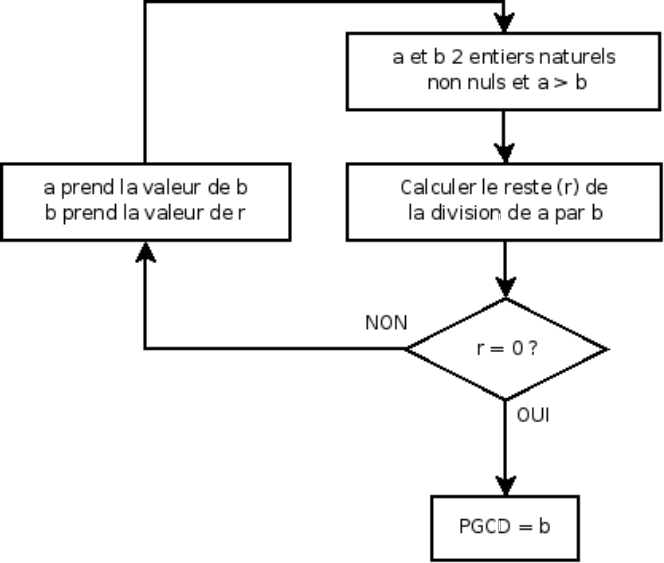
\includegraphics[width=.45\textwidth]{images/algo_euclide}
\end{center}
%\subsection{Recherche des nombres premiers -- Crible d'Ératosthène}
\subsection{Calcul de puissance}
\subsubsection{Algorithme naïf}

\begin{py}
\begin{python}
def exponentiation_naive(x,n):
    """
    Renvoie x* *n par la methode naive.
    Keyword arguments:
    Entrées : 
        x, flt : un nombre réel
        n, int : un nombre entier
    Sortie : 
        res,flt : resultat
    """
    res = 1
    while n>=1:
        res = res * x
        n=n-1
    return res
\end{python}
\end{py}

\subsubsection{Exponentiation rapide itérative}
\begin{py}
\begin{python}
def exponentiation_rapide_iteratif(x,n):
    """ 
    Renvoie x**n par la methode d'exponentiation rapide.
    Keyword arguments:
    Entrées : 
        x, flt : un nombre réel
        n, int : un nombre entier
    Sortie : 
        res,flt : resultat
    """
    if n==0 :
        return 1
    else :
        res = 1
        a = x
        while n>0:
            if n%2 == 1:
                res = res*a
            a=a*a
            n=int(n/2)
        return res
\end{python}
\end{py}


%\section{Calcul d'un polynôme}
%\subsection{Algorithme naïf}
%\subsection{Méthode de Horner}

\begin{thebibliography}{2}
\bibitem{pb}{Patrick Beynet, Cours d'informatique de CPGE, Lycée Rouvière de Toulon, UPSTI.}
\bibitem{ap}{Adrien Petri et Laurent Deschamps, Cours d'informatique de CPGE, Lycée Rouvière de Toulon.}
\bibitem{di}{Damien Iceta, Cours d'informatique de CPGE, Lycée Gustave Eiffel de Cachan, UPSTI.}
\bibitem{wack}{Benjamin WACK, Sylvain CONCHON, Judicaël COURANT, Marc DE FALCO, Gilles DOWEK, Jean-Christophe FILLIÂTRE, Stéphane GONNORD, 
Informatique pour tous en classes préparatoires aux grandes écoles, 
Éditions Eyrolles.}
\end{thebibliography}
\end{document}


 